\chapter{Results}
\label{chap:results}

All the algorithms were run with hyperparameters from chpater \ref{chap:hyperparameters}. Each configuration run a hundred times and the plotted values are mean of specified metric. Results in higher resolution are in the attachment.



%%%%%%%%%%%%%%%%%
%%             %%
%%   GENETIC   %%
%%             %%
%%%%%%%%%%%%%%%%%
\begin{figure}[ht!]
    \centering
    \begin{minipage}[t]{0.9\textwidth}
        \begin{minipage}[t]{0.48\textwidth}
            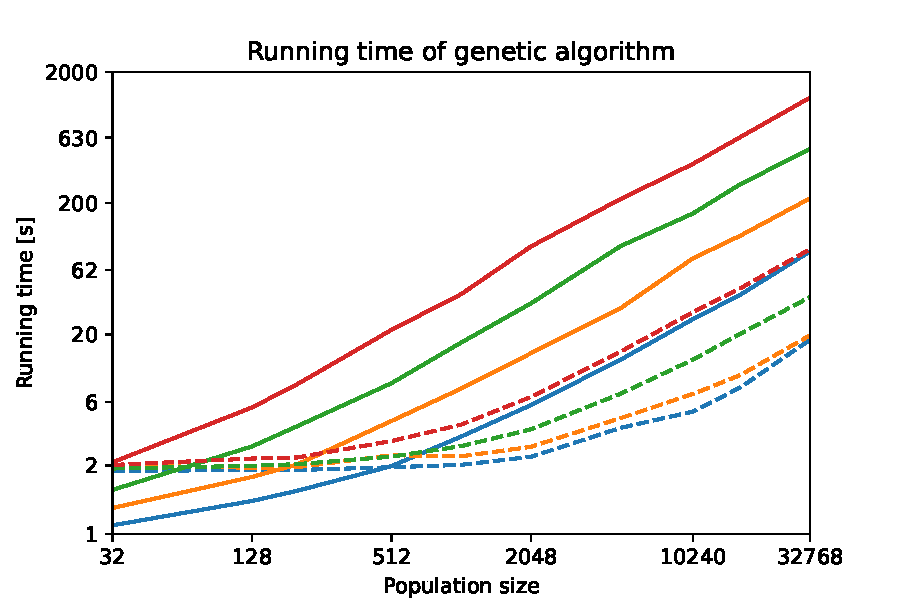
\includegraphics[width=\textwidth]{img/runs/time_ga.pdf}
        \end{minipage}
        \begin{minipage}[t]{0.48\textwidth}
            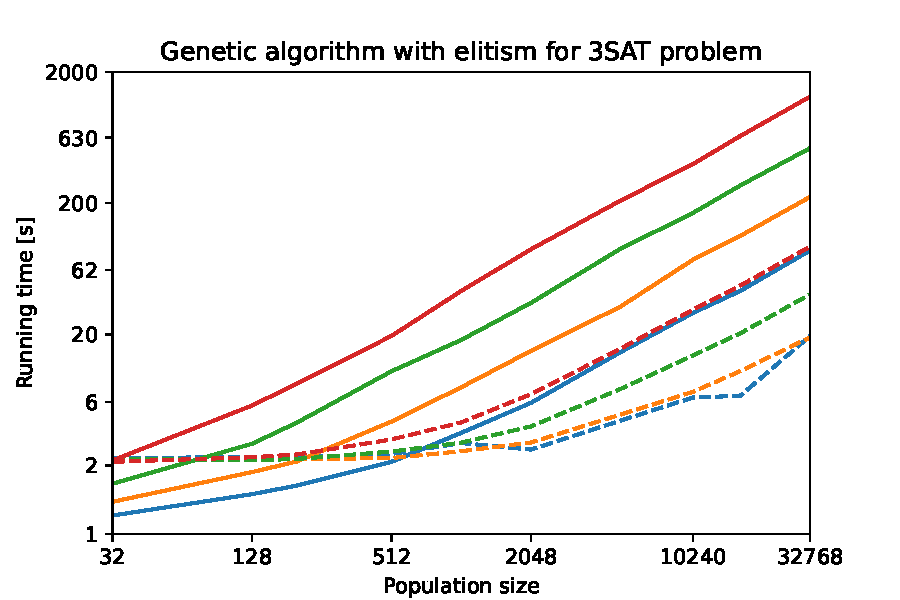
\includegraphics[width=\textwidth]{img/runs/time_ga_elitism.pdf}
        \end{minipage}
    \end{minipage}

    \begin{minipage}[t]{0.7\textwidth}
        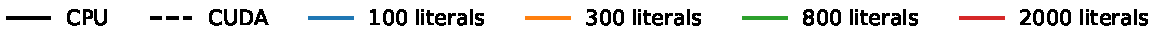
\includegraphics[width=\textwidth]{img/runs/time_ga_legend.pdf}
    \end{minipage}

    \caption[Genetic algorithm running time with and without elitism]{Running time of \acrlong{acc:ga} with and without elitism for \acrshort{acc:3sat} problem. All the formulas have been satisfiable and had $4.5$ times more clauses than literals. The algorithm run for $1000$ generations.}
    \label{meas:garuntime}
\end{figure}

\begin{figure}[ht!]
    \centering
    \begin{minipage}[t]{0.9\textwidth}
        \begin{minipage}[t]{0.48\textwidth}
            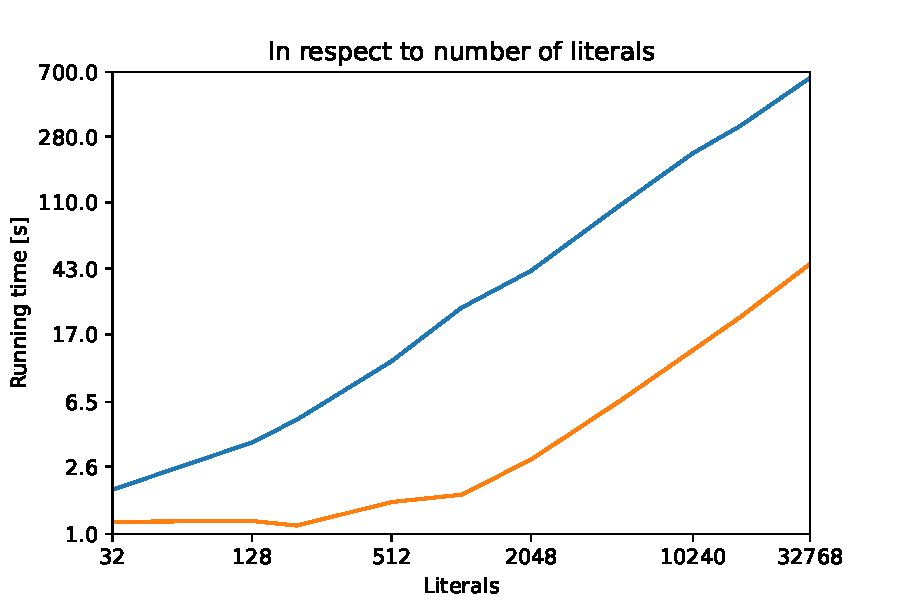
\includegraphics[width=\textwidth]{img/runs/time_ga_varcount.pdf}
        \end{minipage}
        \begin{minipage}[t]{0.48\textwidth}
            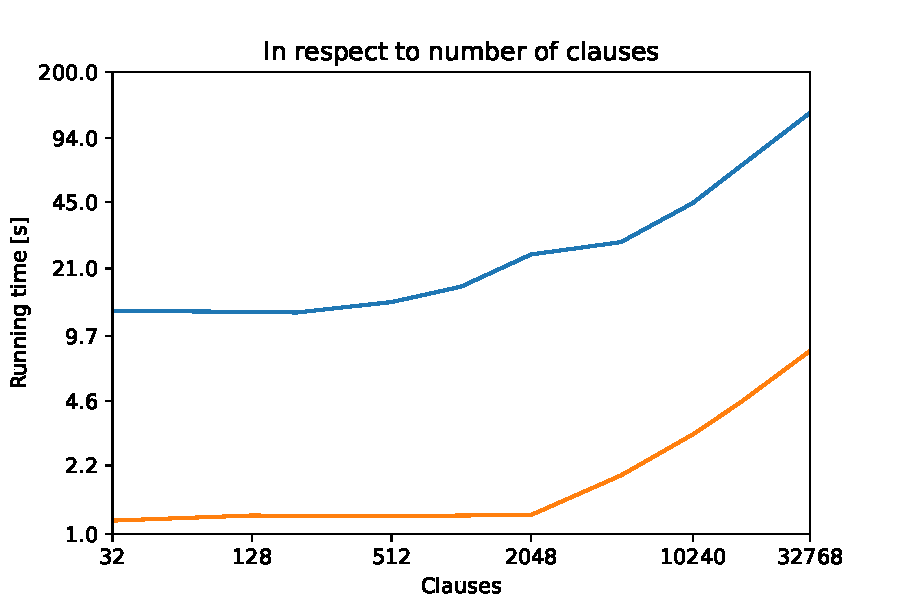
\includegraphics[width=\textwidth]{img/runs/time_ga_clausecount.pdf}
        \end{minipage}
    \end{minipage}

    \begin{minipage}[t]{0.15\textwidth}
        
\includegraphics[width=\textwidth]{img/runs/time_ga_clausecount_legend.pdf}
    \end{minipage}

    \caption[Running time of Genetic Algorithm in respect to problem size]{Running time of \acrlong{acc:ga} for \acrshort{acc:3sat} problem in respect to problem size. On the left in respect to number of literals with $4.5$ times the number of clauses, and in respect to number of clauses for $2000$ literals on the right. All the formulas have been satisfiable and measurements are done for population size $1000$. The algorithm run for $1000$ generations.}
    \label{meas:garuntimeproblemsize}
\end{figure}

\begin{figure}[ht!]
    \begin{minipage}[t]{0.32\textwidth}
        \centering
        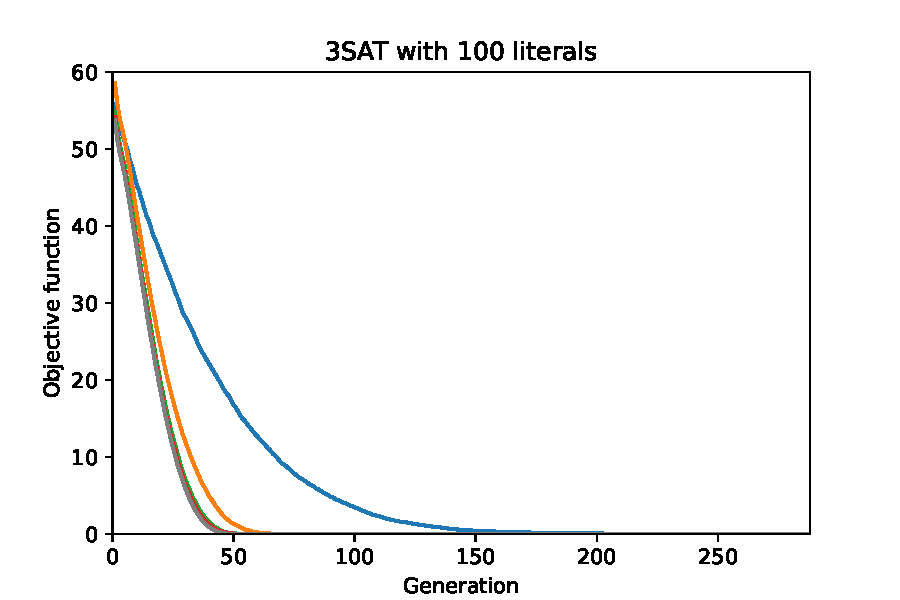
\includegraphics[width=\textwidth]{img/runs/fitness_ga_3SAT_d100.pdf}
    \end{minipage}
    \hfill
    \begin{minipage}[t]{0.32\textwidth}
        \centering
        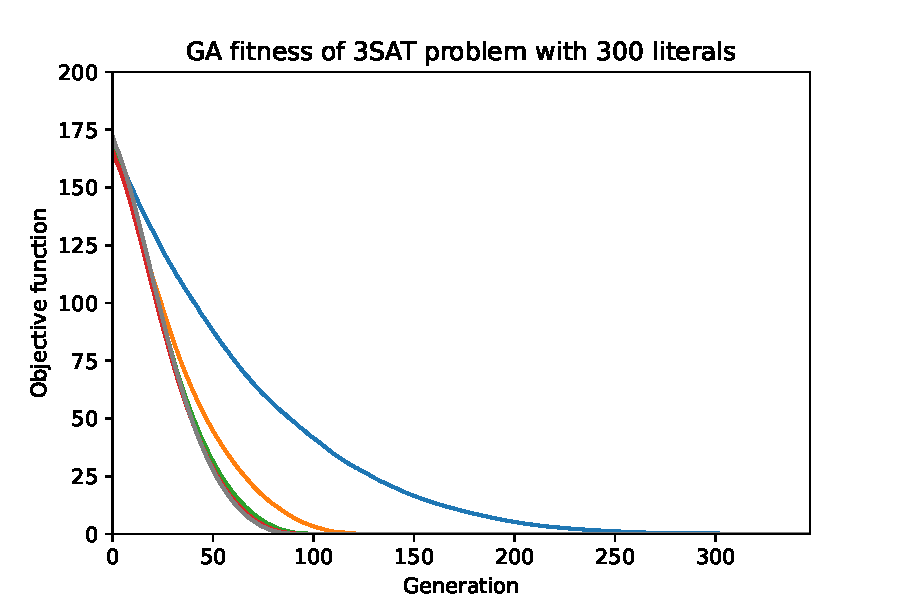
\includegraphics[width=\textwidth]{img/runs/fitness_ga_3SAT_d300.pdf}
    \end{minipage}
    \hfill
    \begin{minipage}[t]{0.32\textwidth}
        \centering
        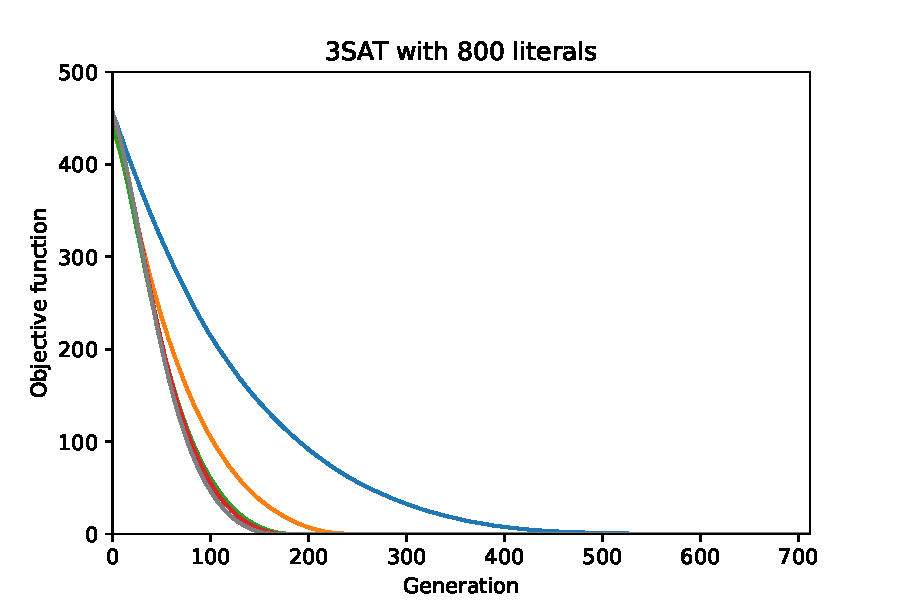
\includegraphics[width=\textwidth]{img/runs/fitness_ga_3SAT_d800.pdf}
    \end{minipage}

    \begin{minipage}[t]{0.32\textwidth}
        \centering
        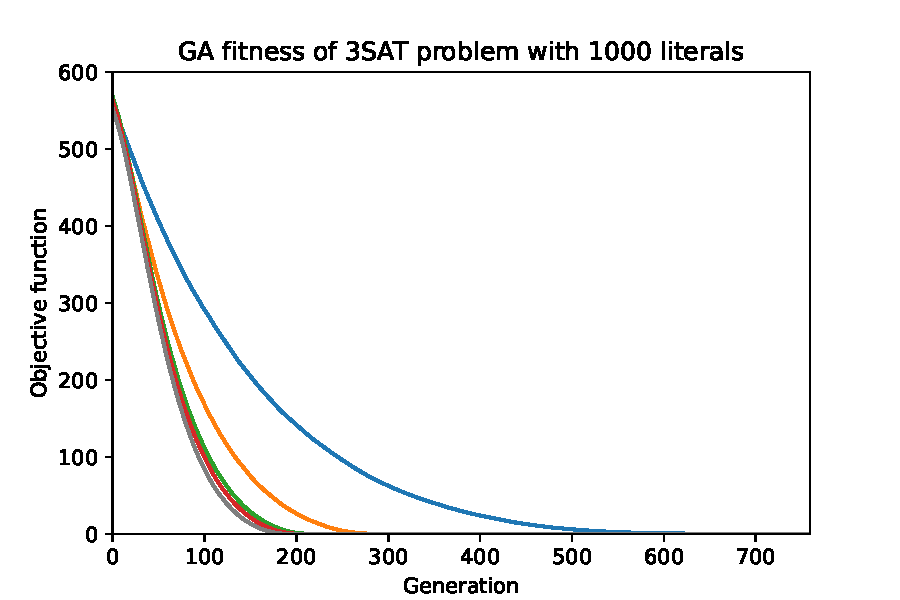
\includegraphics[width=\textwidth]{img/runs/fitness_ga_3SAT_d1000.pdf}
    \end{minipage}
    \hfill
    \begin{minipage}[t]{0.32\textwidth}
        \centering
        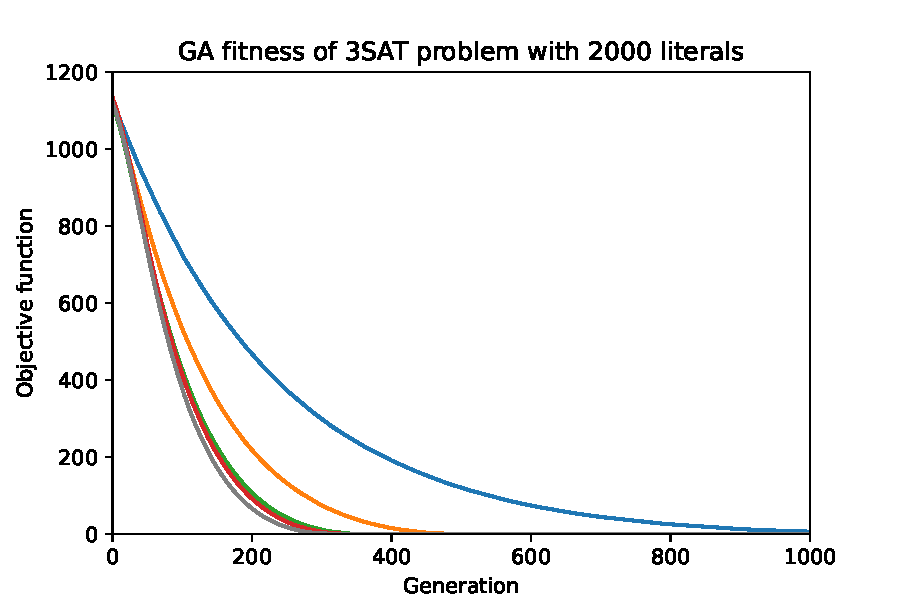
\includegraphics[width=\textwidth]{img/runs/fitness_ga_3SAT_d2000.pdf}
    \end{minipage}
    \hfill
    \begin{minipage}[t]{0.32\textwidth}
        \centering
        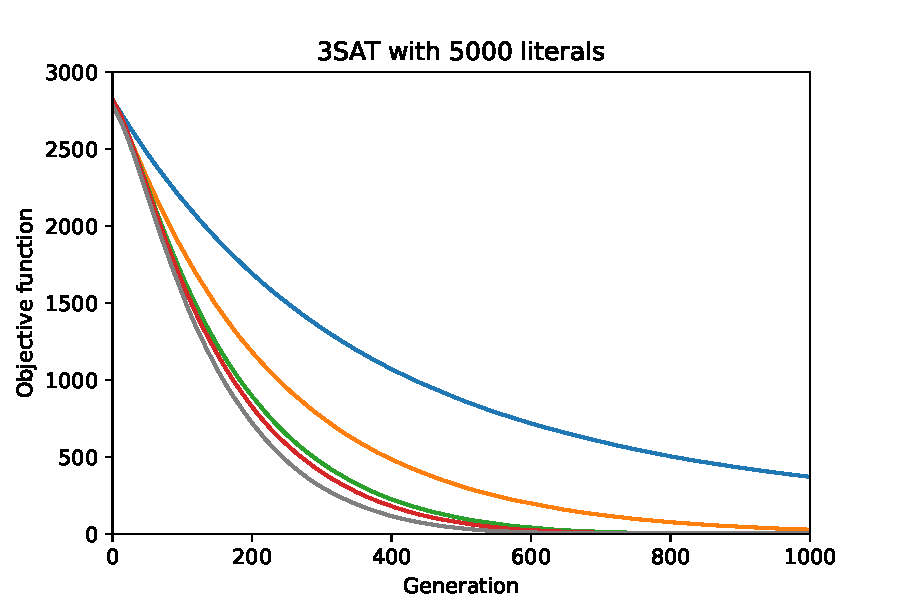
\includegraphics[width=\textwidth]{img/runs/fitness_ga_3SAT_d5000.pdf}
    \end{minipage}

    \begin{minipage}{\textwidth}
        \centering
        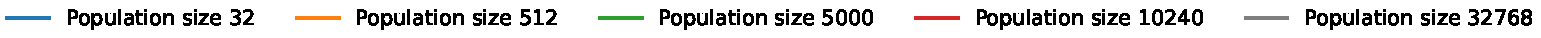
\includegraphics[width=0.8\textwidth]{img/runs/fitness_ga_3SAT_legend.pdf}
    \end{minipage}

    \caption[Fitness of genetic algorithm]{Fitness of \acrlong{acc:ga} on \acrshort{acc:3sat} problem. Algorithm run for maximum of $1000$ generations and had $4.5$ times number of clauses than the literals. The graphs show $0.05$ quantile of the fitness value in the population.}
    \label{meas:gafitness}
\end{figure}

\begin{figure}[ht!]
    \begin{minipage}[t]{0.32\textwidth}
        \centering
        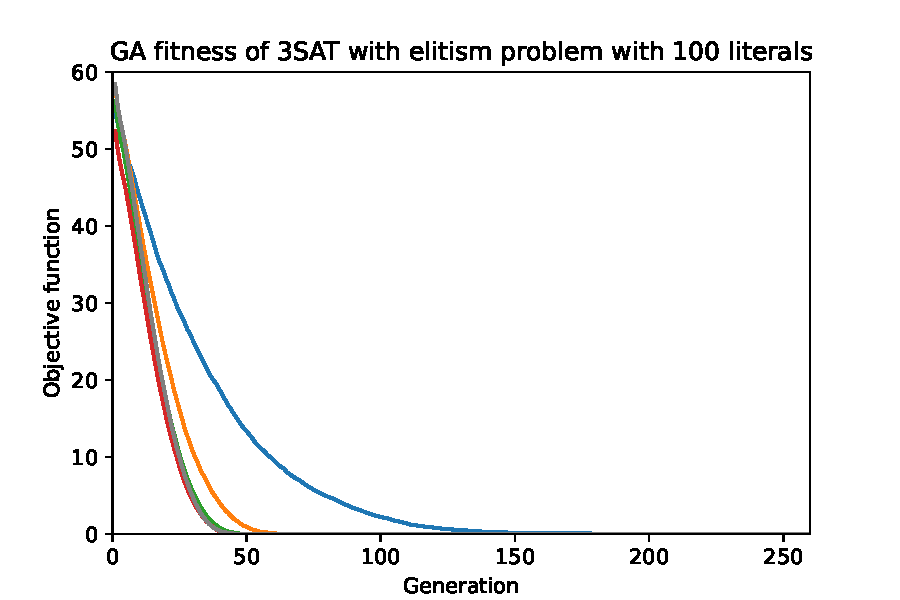
\includegraphics[width=\textwidth]{img/runs/fitness_ga_elitism_3SAT_d100.pdf}
    \end{minipage}
    \hfill
    \begin{minipage}[t]{0.32\textwidth}
        \centering
        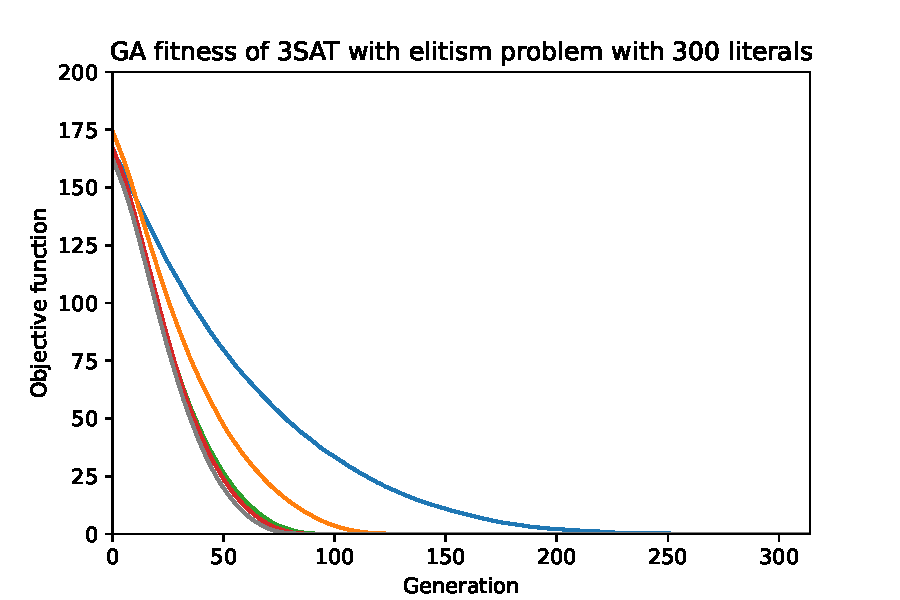
\includegraphics[width=\textwidth]{img/runs/fitness_ga_elitism_3SAT_d300.pdf}
    \end{minipage}
    \hfill
    \begin{minipage}[t]{0.32\textwidth}
        \centering
        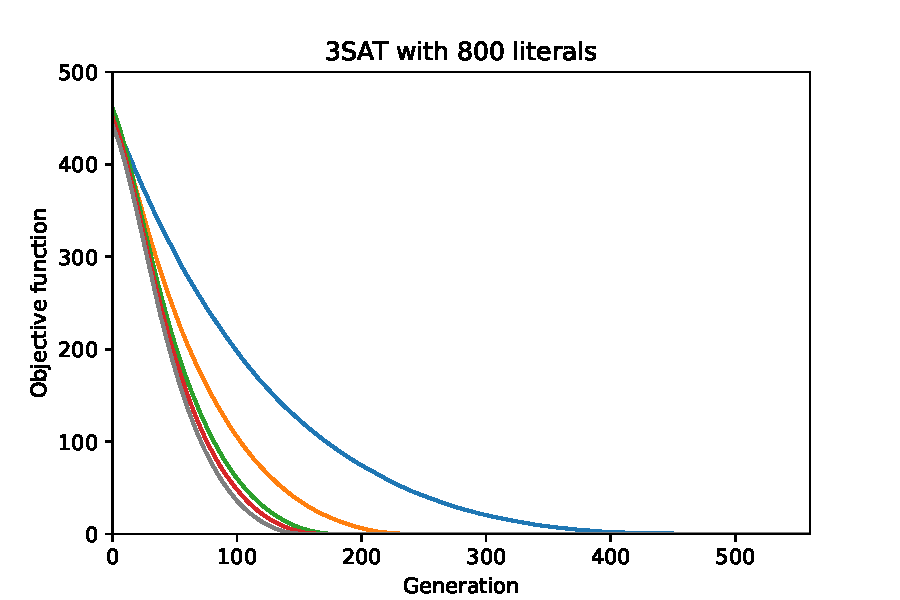
\includegraphics[width=\textwidth]{img/runs/fitness_ga_elitism_3SAT_d800.pdf}
    \end{minipage}

    \begin{minipage}[t]{0.32\textwidth}
        \centering
        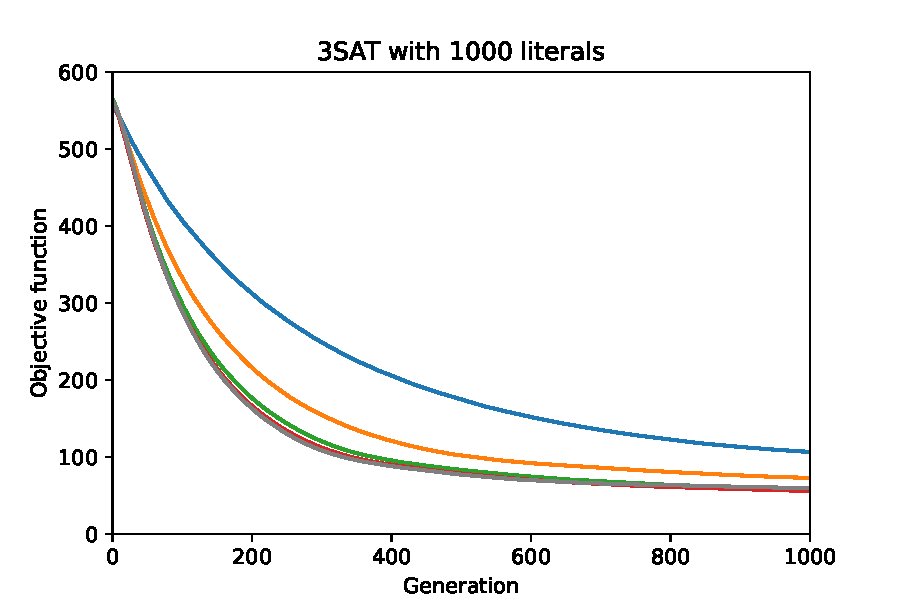
\includegraphics[width=\textwidth]{img/runs/fitness_ga_elitism_3SAT_d1000.pdf}
    \end{minipage}
    \hfill
    \begin{minipage}[t]{0.32\textwidth}
        \centering
        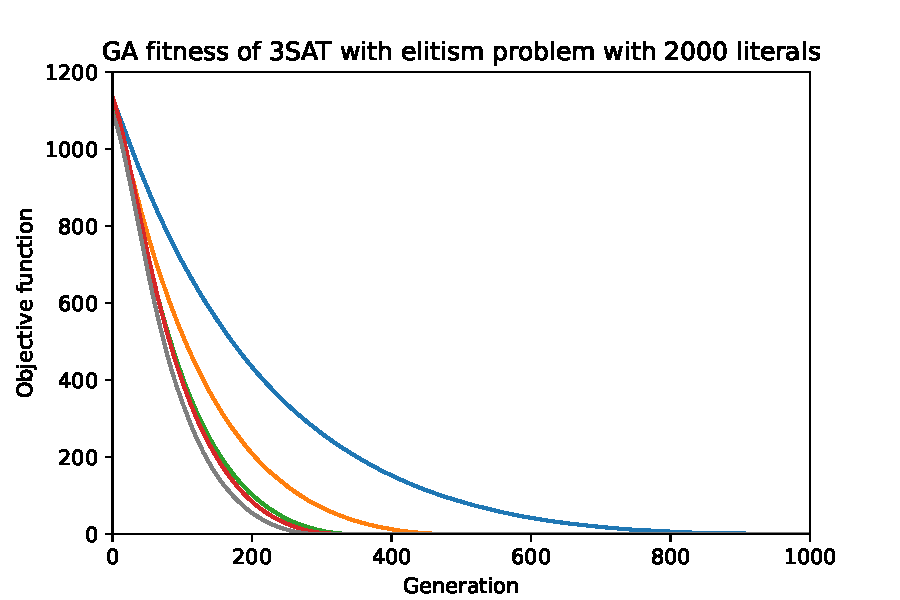
\includegraphics[width=\textwidth]{img/runs/fitness_ga_elitism_3SAT_d2000.pdf}
    \end{minipage}
    \hfill
    \begin{minipage}[t]{0.32\textwidth}
        \centering
        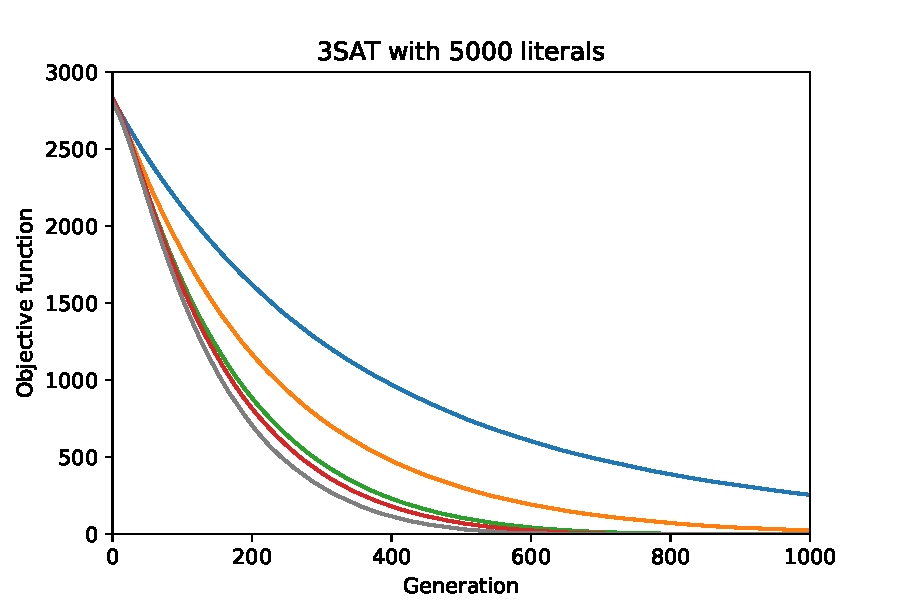
\includegraphics[width=\textwidth]{img/runs/fitness_ga_elitism_3SAT_d5000.pdf}
    \end{minipage}

    \begin{minipage}{\textwidth}
        \centering
        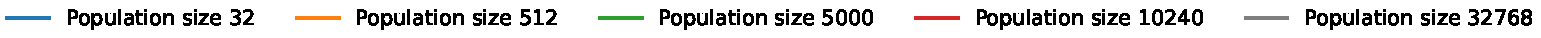
\includegraphics[width=0.8\textwidth]{img/runs/fitness_ga_3SAT_legend.pdf}
    \end{minipage}

    \caption[Fitness of genetic algorithm with elitism]{Fitness of \acrlong{acc:ga} with elitism on \acrshort{acc:3sat} problem. Algorithm run for maximum of $1000$ generations and had $4.5$ times number of clauses than the literals. The graphs show $0.05$ quantile of the fitness value in the population.}
    \label{meas:gafitnesselite}
\end{figure}





%%%%%%%%%%%%%%%%%
%%             %%
%%   SCALING   %%
%%             %%
%%%%%%%%%%%%%%%%%

\begin{figure}[ht!]
    \centering
    \begin{minipage}[t]{0.9\textwidth}
        \begin{minipage}[t]{0.48\textwidth}
            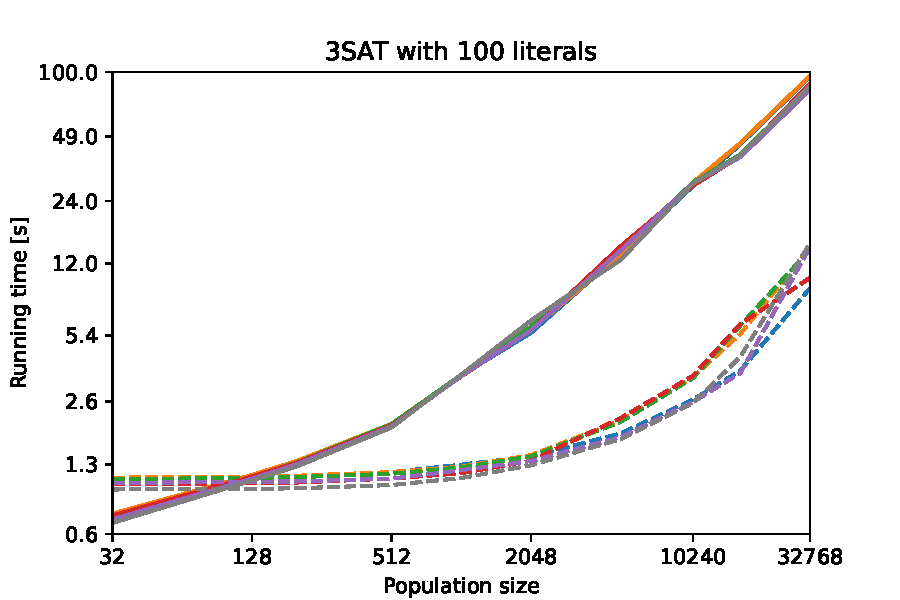
\includegraphics[width=\textwidth]{img/runs/time_ga_scale_100l.pdf}
        \end{minipage}
        \begin{minipage}[t]{0.48\textwidth}
            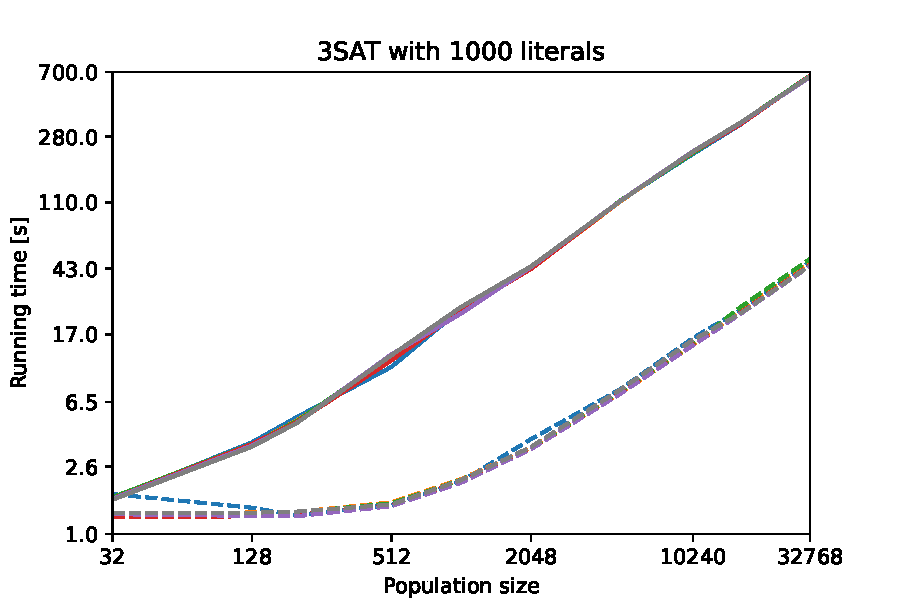
\includegraphics[width=\textwidth]{img/runs/time_ga_scale_1000l.pdf}
        \end{minipage}
    \end{minipage}

    \begin{minipage}[t]{0.9\textwidth}
        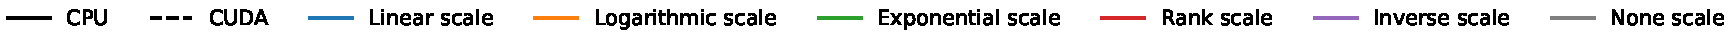
\includegraphics[width=\textwidth]{img/runs/time_ga_scale_legend.pdf}
    \end{minipage}

    \caption[Running time of genetic algorithm with various scale operators]{Running time of \acrlong{acc:ga} with various fitness scale operators. The algorithm were solving \acrshort{acc:3sat} problem with $100$ (left) resp. $1000$ (right) literals and $450$, resp. $4500$ clauses. The algorithm run for $1000$ generations.}
    \label{meas:scale}
\end{figure}



%%%%%%%%%%%%%%%%%%%
%%               %%
%%   SELECTION   %%
%%               %%
%%%%%%%%%%%%%%%%%%%

\begin{figure}[ht!]
    \centering
    \begin{minipage}[t]{0.9\textwidth}
        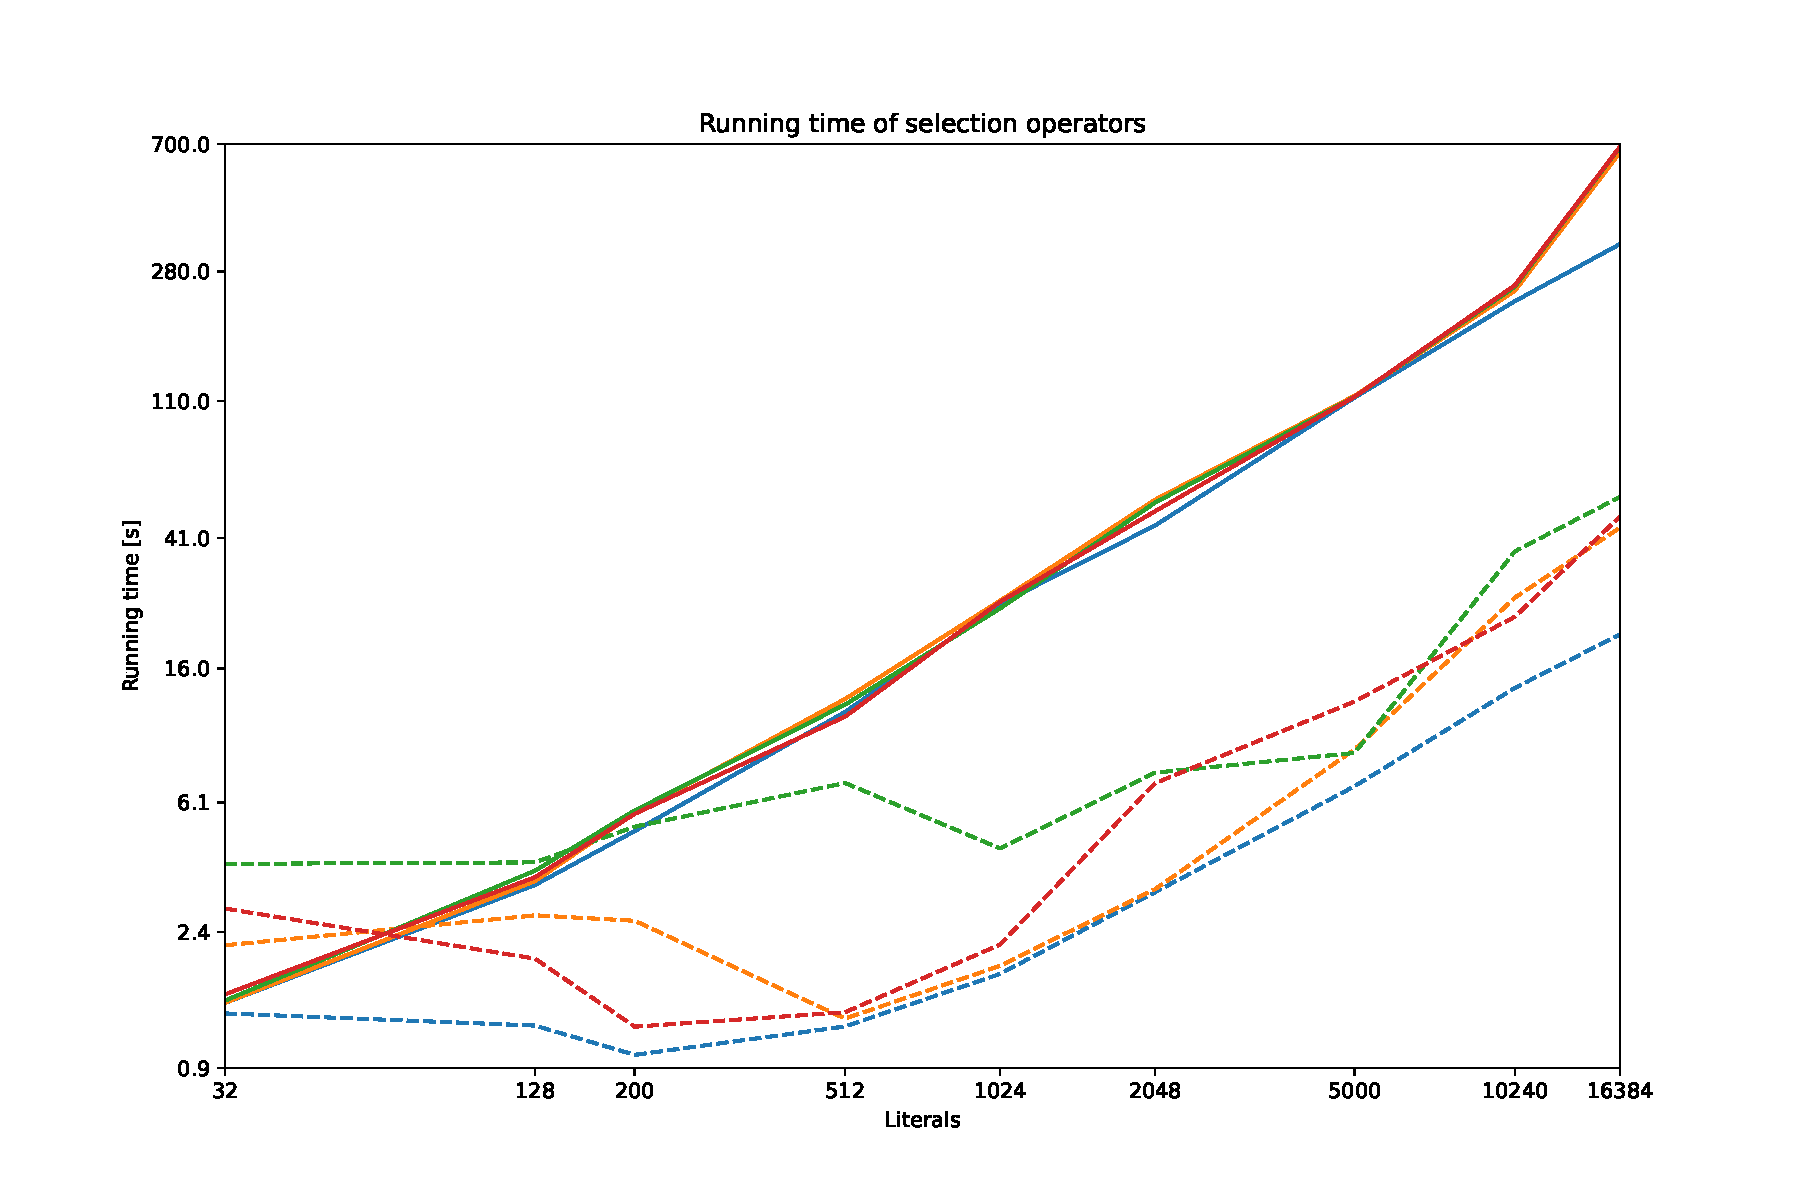
\includegraphics[width=\textwidth]{img/runs/time_ga_selections.pdf}
    \end{minipage}

    \begin{minipage}[t]{0.9\textwidth}
        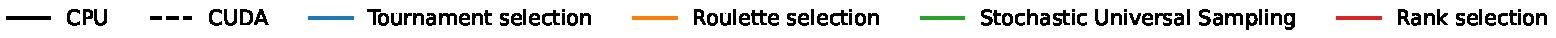
\includegraphics[width=\textwidth]{img/runs/time_ga_selections_legend.pdf}
    \end{minipage}

    \caption[Running time of selection operators]{Running time of \acrlong{acc:ga} with various selection operators. The algorithm were solving \acrshort{acc:3sat} problem with $1000$ literals and $4500$ clauses, and run for $1000$ generations.}
    \label{meas:selection}
\end{figure}




%%%%%%%%%%%%%%%%%%%%%%%%%%
%%                      %%
%%   CPP IMPLEMENTACE   %%
%%                      %%
%%%%%%%%%%%%%%%%%%%%%%%%%%

\begin{figure}[ht!]
    \centering
    \begin{minipage}[t]{0.9\textwidth}
        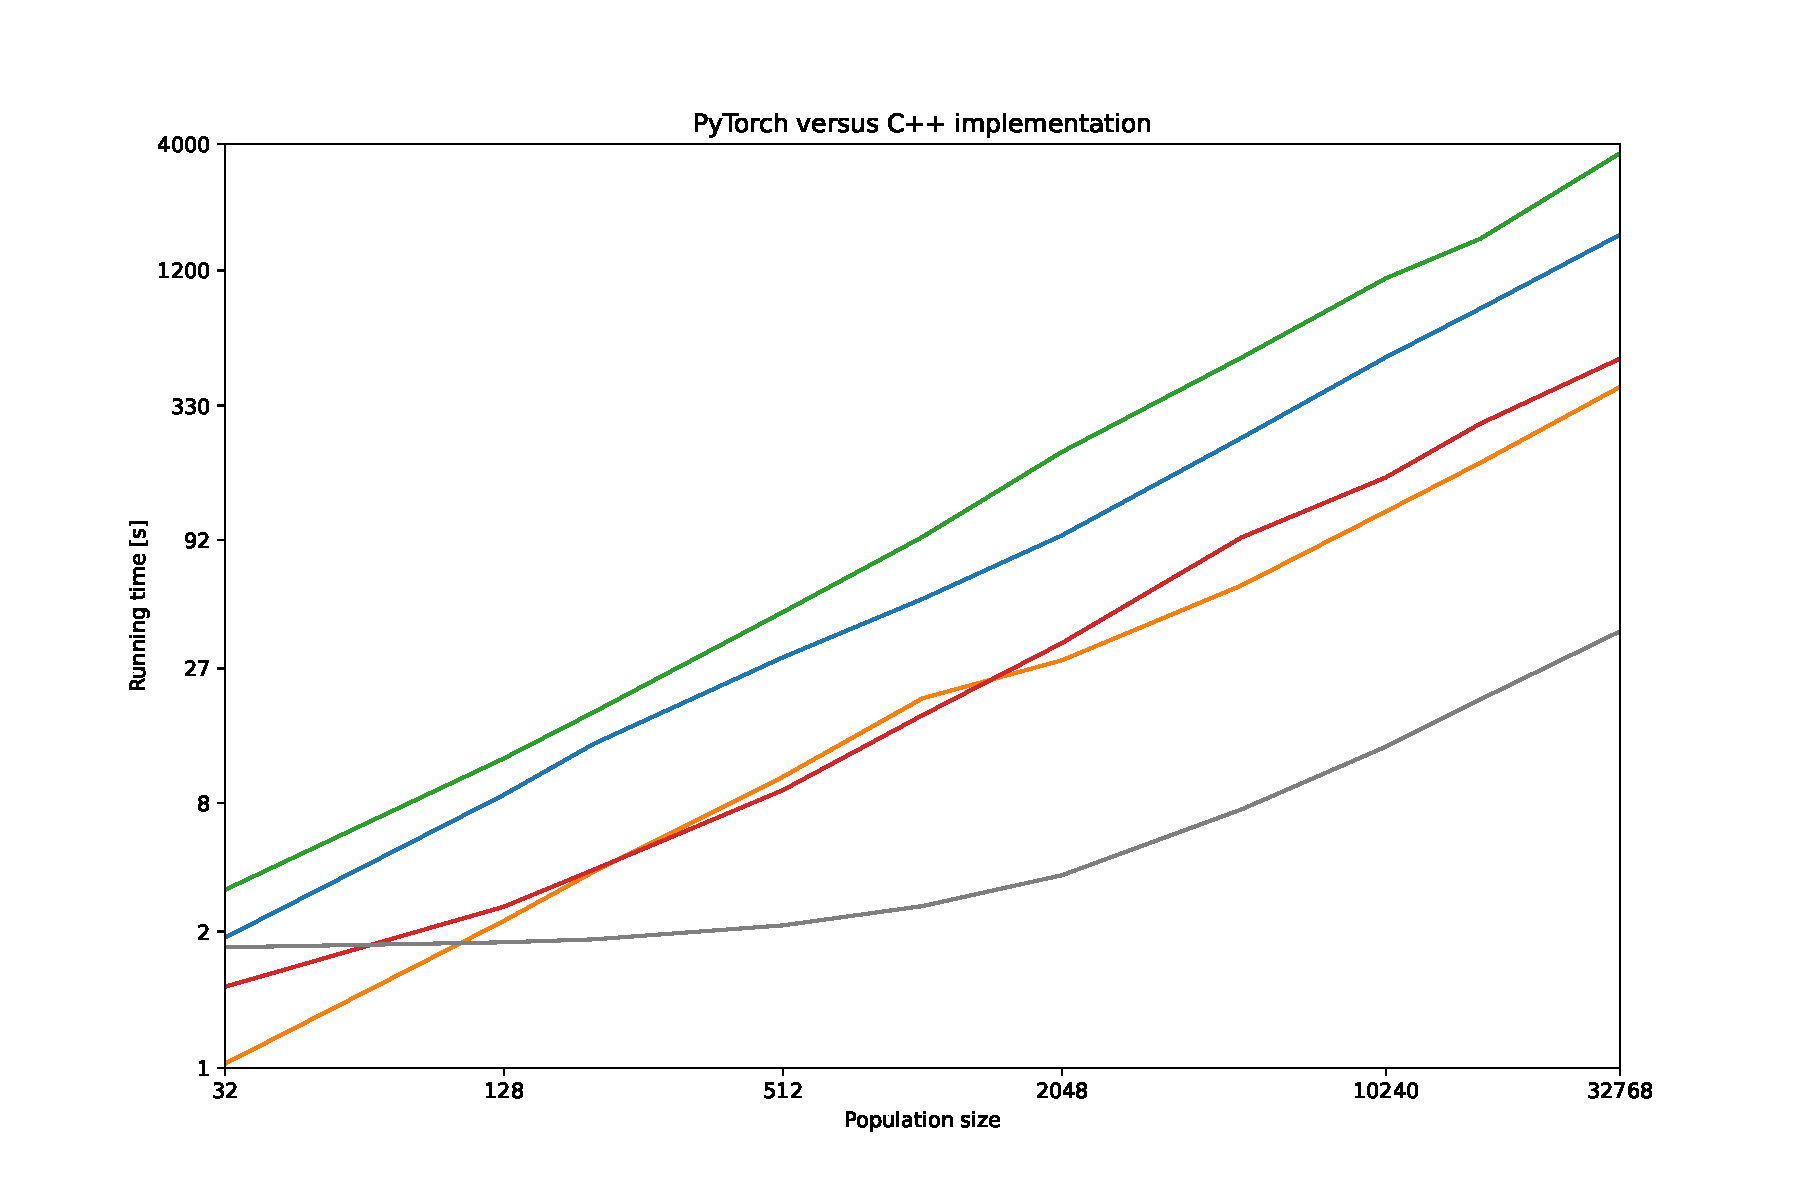
\includegraphics[width=\textwidth]{img/runs/time_ga_c.pdf}
    \end{minipage}

    \begin{minipage}[t]{0.9\textwidth}
        
\includegraphics[width=\textwidth]{img/runs/time_ga_c_legend.pdf}
    \end{minipage}

    \caption[Comparison of PyTorch and \cpp implementation]{Running time of \acrlong{acc:ga} implemented in PyTorch and \cppns. The algorithm were solving \acrshort{acc:3sat} problem with $800$ literals and $3600$ clauses, and run for $1000$ generations. The \cpp implementation used the master--worker approach to evaluate fitness function in parallel.}
    \label{meas:cimpl}
\end{figure}




%%%%%%%%%%%%%%%%%%%%%%
%%                  %%
%%   ES MUTATIONS   %%
%%                  %%
%%%%%%%%%%%%%%%%%%%%%%
\begin{figure}[ht!]
    \begin{minipage}[t]{0.32\textwidth}
        \centering
        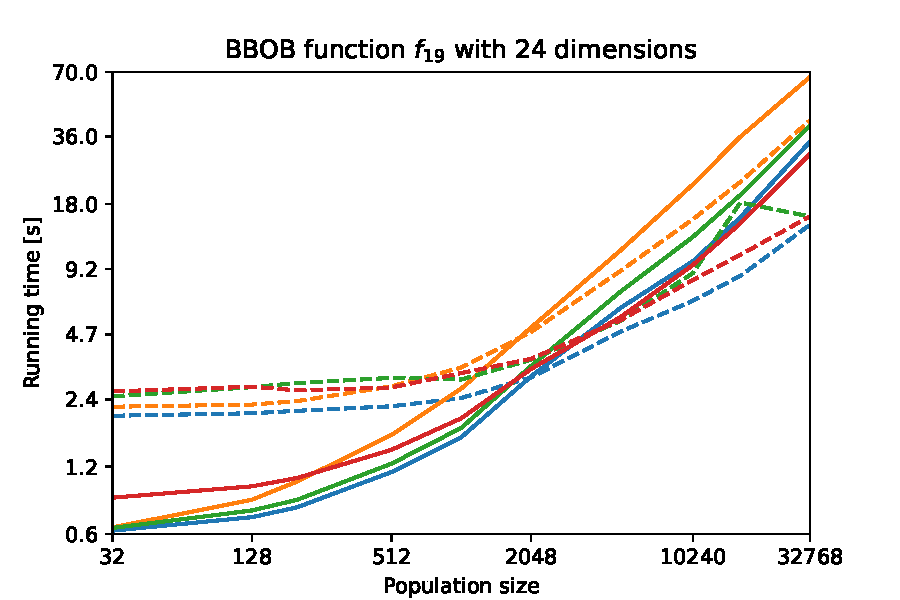
\includegraphics[width=\textwidth]{img/runs/time_es_mutation_fn19_24d.pdf}
    \end{minipage}
    \hfill
    \begin{minipage}[t]{0.32\textwidth}
        \centering
        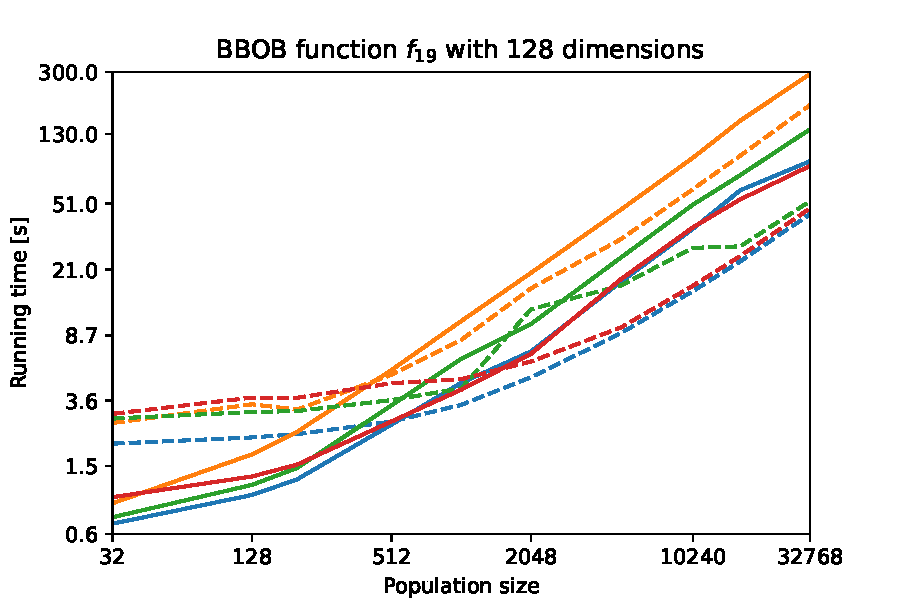
\includegraphics[width=\textwidth]{img/runs/time_es_mutation_fn19_128d.pdf}
    \end{minipage}
    \hfill
    \begin{minipage}[t]{0.32\textwidth}
        \centering
        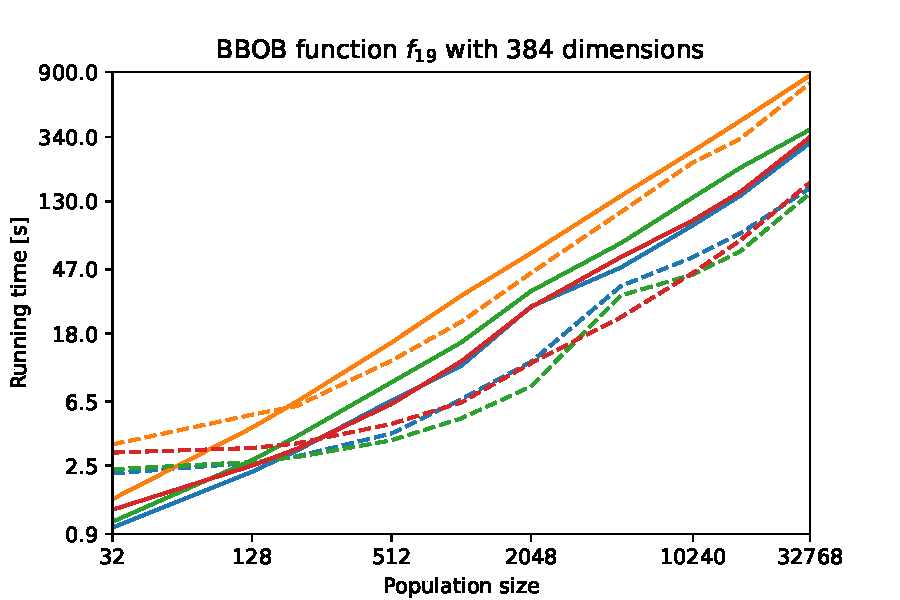
\includegraphics[width=\textwidth]{img/runs/time_es_mutation_fn19_384d.pdf}
    \end{minipage}

    \begin{minipage}[t]{0.32\textwidth}
        \centering
        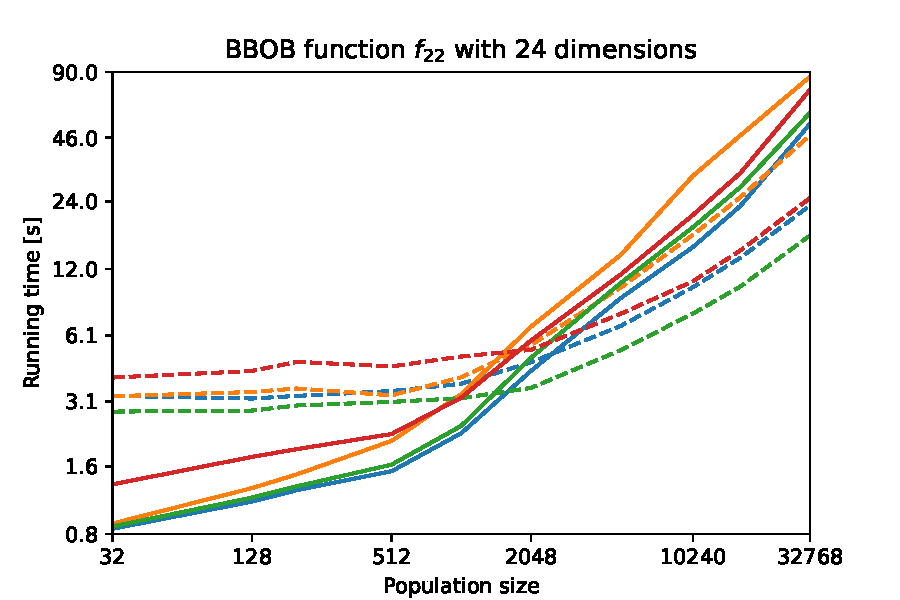
\includegraphics[width=\textwidth]{img/runs/time_es_mutation_fn22_24d.pdf}
    \end{minipage}
    \hfill
    \begin{minipage}[t]{0.32\textwidth}
        \centering
        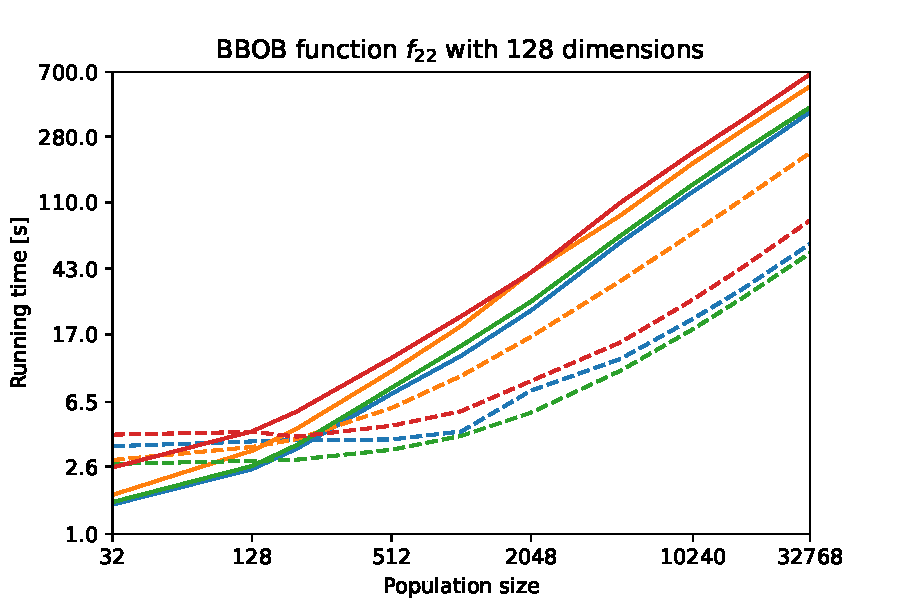
\includegraphics[width=\textwidth]{img/runs/time_es_mutation_fn22_128d.pdf}
    \end{minipage}
    \hfill
    \begin{minipage}[t]{0.32\textwidth}
        \centering
        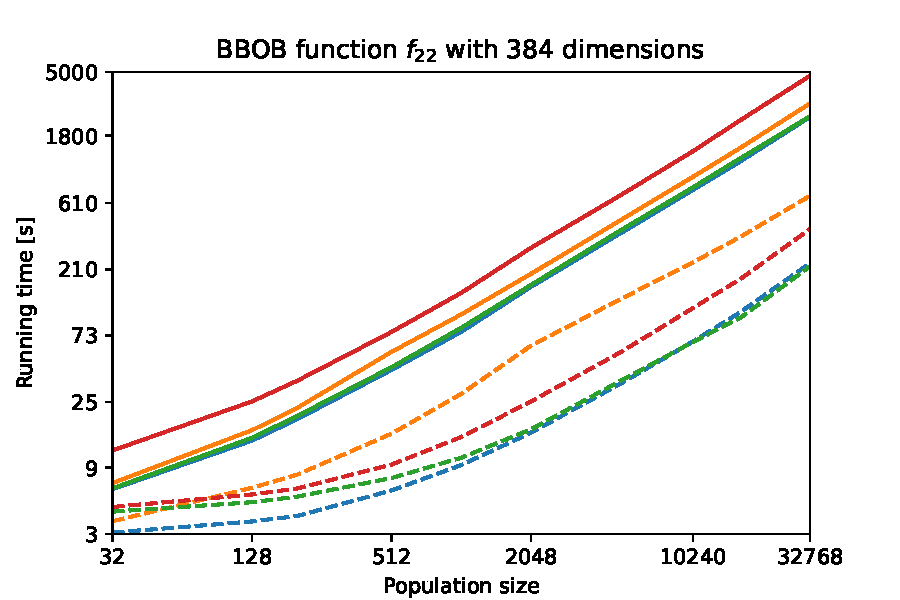
\includegraphics[width=\textwidth]{img/runs/time_es_mutation_fn22_384d.pdf}
    \end{minipage}

    \begin{minipage}{\textwidth}
        \centering
        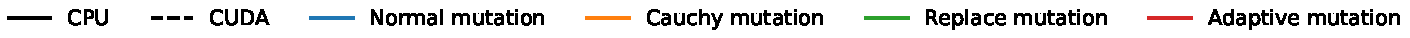
\includegraphics[width=0.8\textwidth]{img/runs/time_es_mutation_legend.pdf}
    \end{minipage}

    \caption[Running time of mutation operators]{Running time of real--coded evolutionary algorithm with various mutation operators. I chose to measure only \acrshort{acc:bbob} functions $f_{19}$ and $f_{22}$. Algorithm used hyperparameters specified in table \ref{tab:esmutationhyperparmarameters} and run for $1000$ generations.}
    \label{meas:muttime}
\end{figure}



\begin{figure}[ht!]
    \begin{minipage}[t]{0.32\textwidth}
        \centering
        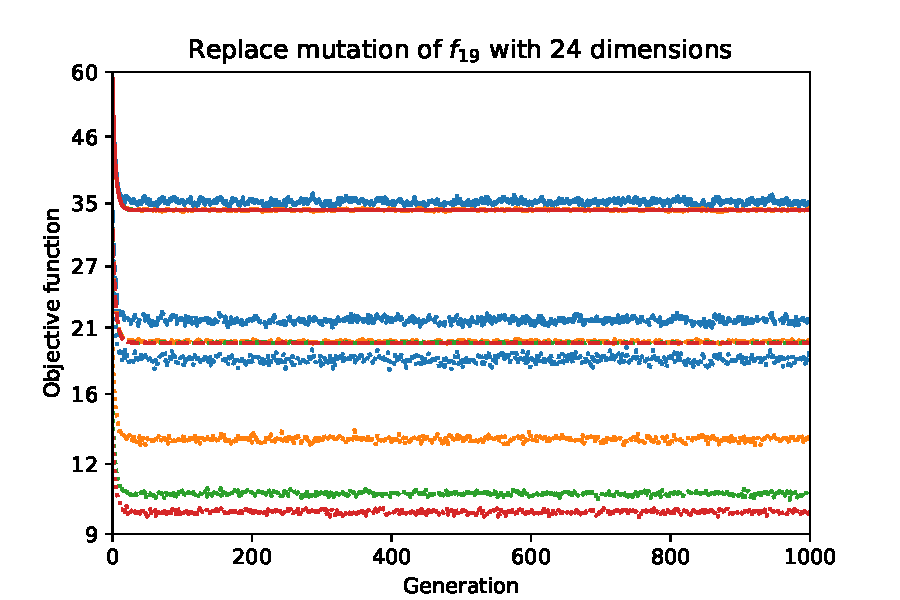
\includegraphics[width=\textwidth]{img/runs/fitness_es_mutation_f19_dim24_ReplaceUniform.pdf}
    \end{minipage}
    \hfill
    \begin{minipage}[t]{0.32\textwidth}
        \centering
        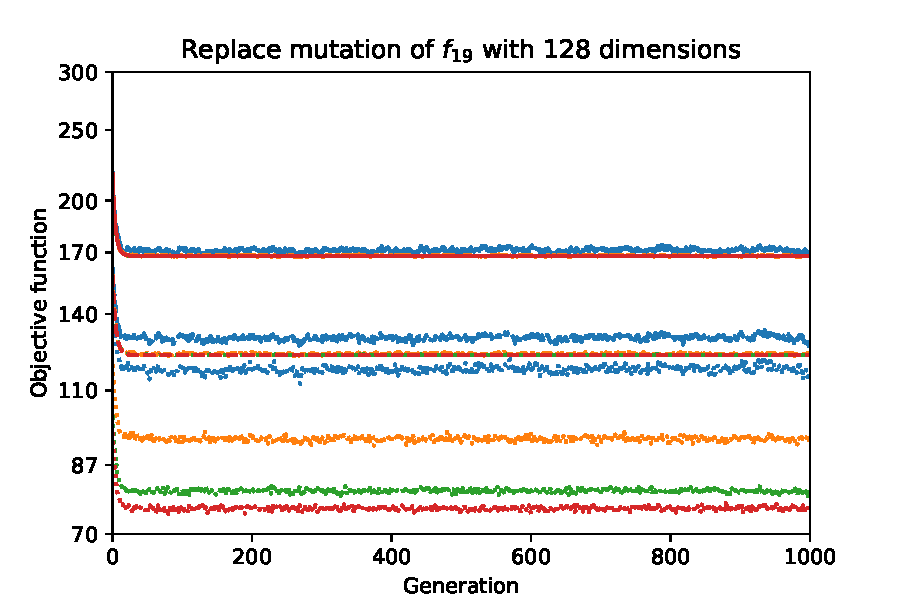
\includegraphics[width=\textwidth]{img/runs/fitness_es_mutation_f19_dim128_ReplaceUniform.pdf}
    \end{minipage}
    \hfill
    \begin{minipage}[t]{0.32\textwidth}
        \centering
        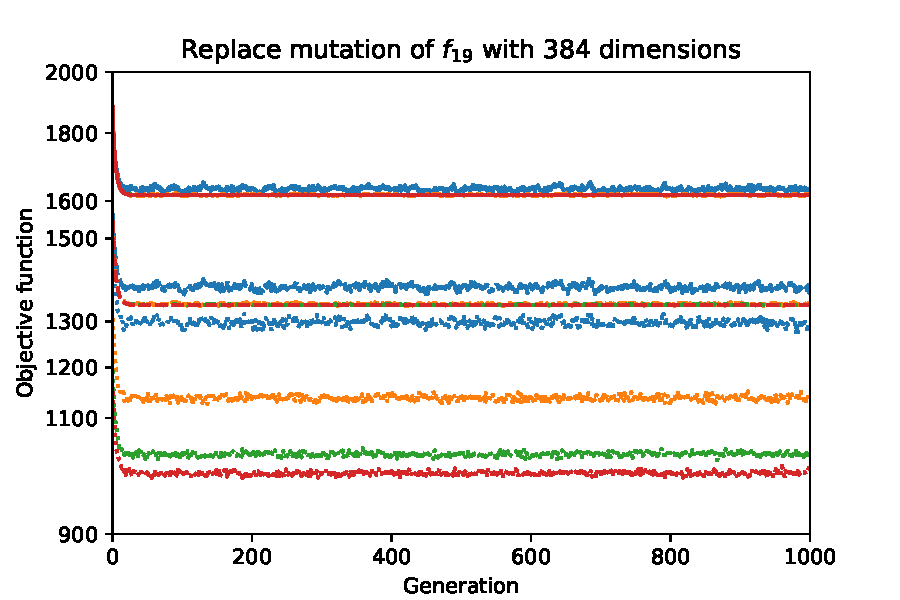
\includegraphics[width=\textwidth]{img/runs/fitness_es_mutation_f19_dim384_ReplaceUniform.pdf}
    \end{minipage}

    \begin{minipage}[t]{0.32\textwidth}
        \centering
        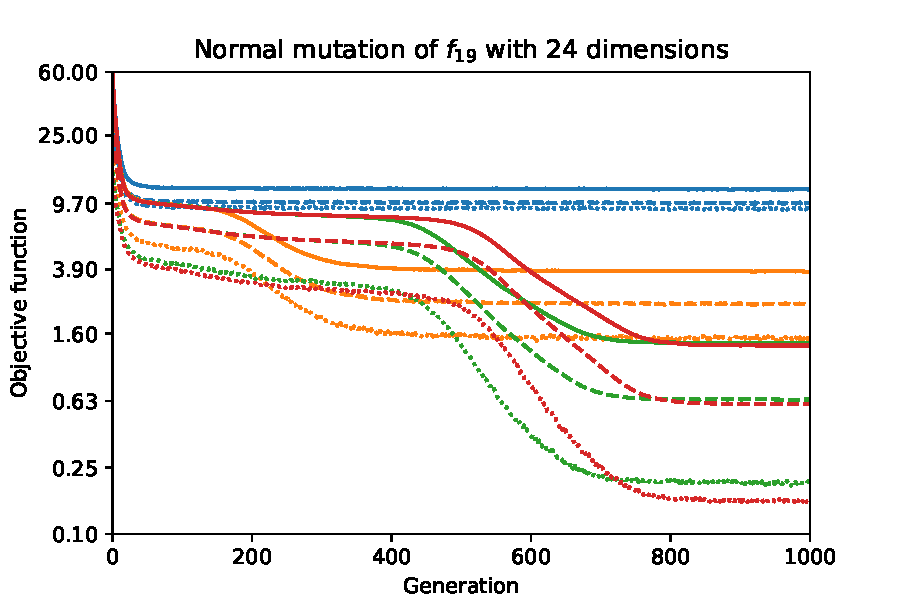
\includegraphics[width=\textwidth]{img/runs/fitness_es_mutation_f19_dim24_AddFromNormal.pdf}
    \end{minipage}
    \hfill
    \begin{minipage}[t]{0.32\textwidth}
        \centering
        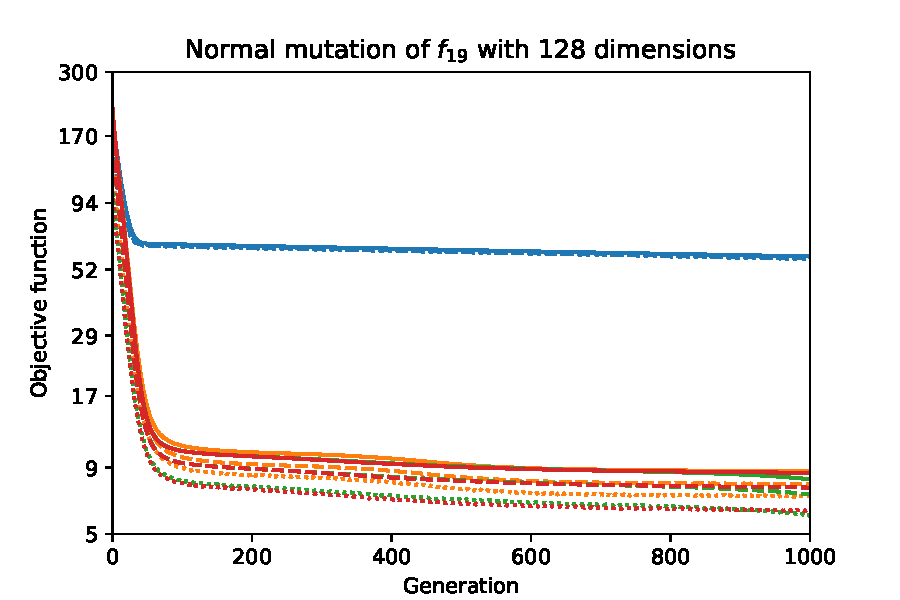
\includegraphics[width=\textwidth]{img/runs/fitness_es_mutation_f19_dim128_AddFromNormal.pdf}
    \end{minipage}
    \hfill
    \begin{minipage}[t]{0.32\textwidth}
        \centering
        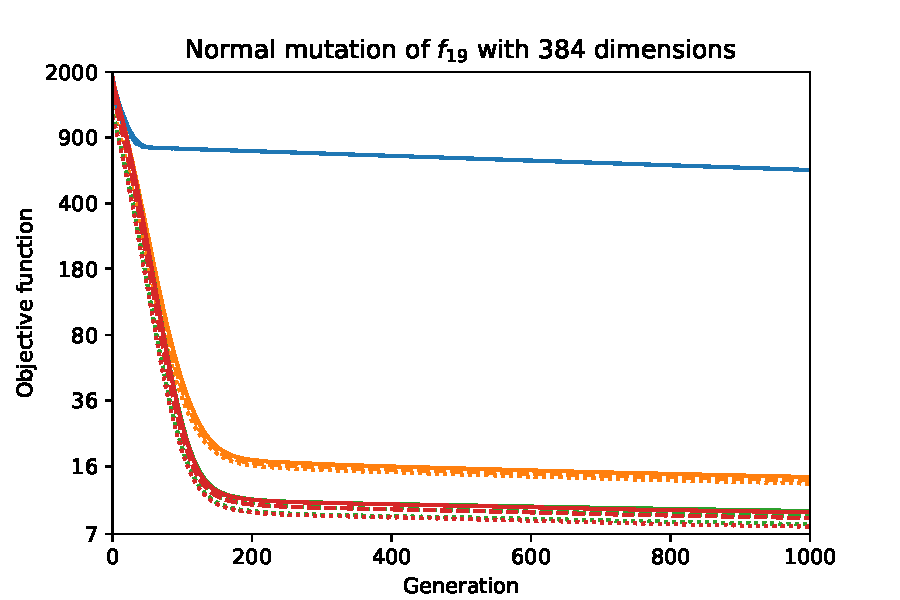
\includegraphics[width=\textwidth]{img/runs/fitness_es_mutation_f19_dim384_AddFromNormal.pdf}
    \end{minipage}

    \begin{minipage}[t]{0.32\textwidth}
        \centering
        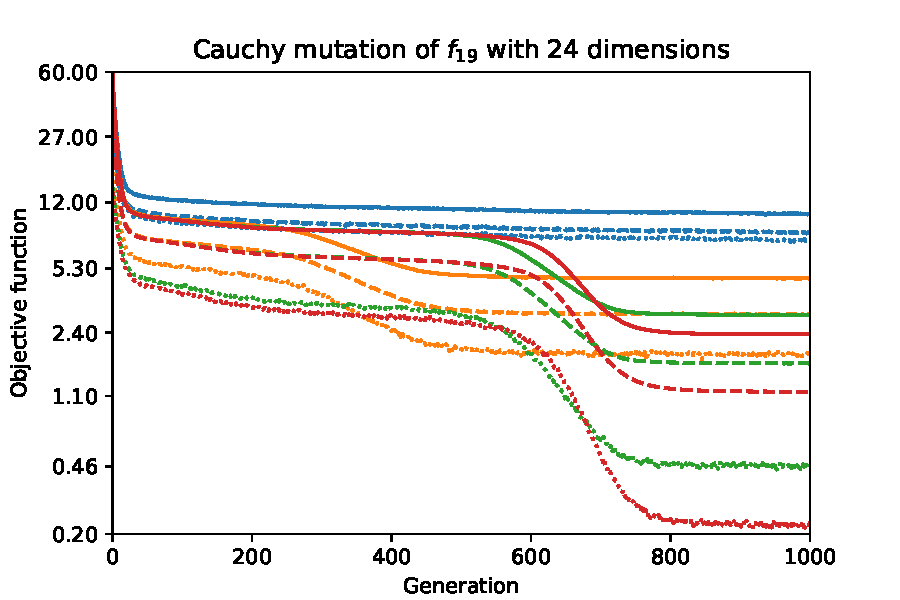
\includegraphics[width=\textwidth]{img/runs/fitness_es_mutation_f19_dim24_AddFromCauchy.pdf}
    \end{minipage}
    \hfill
    \begin{minipage}[t]{0.32\textwidth}
        \centering
        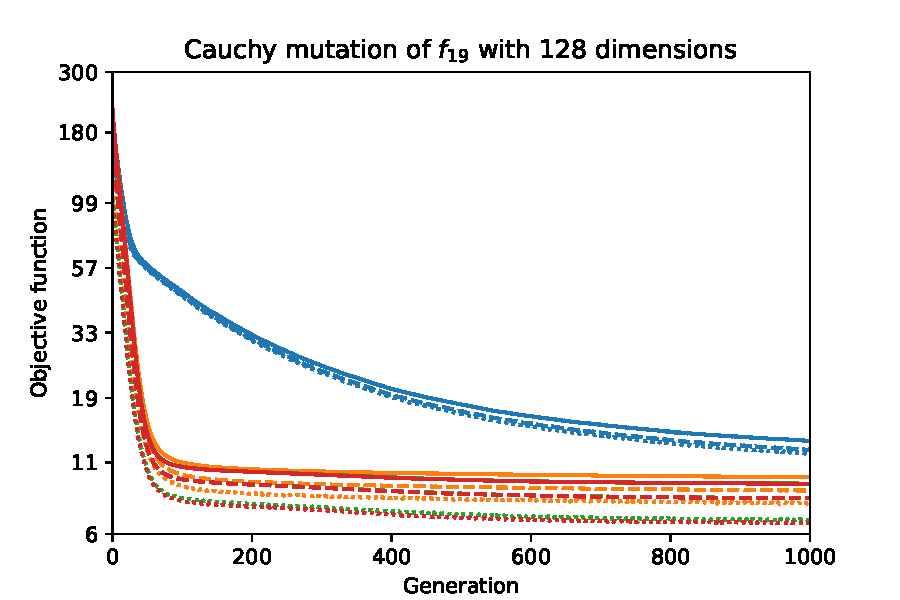
\includegraphics[width=\textwidth]{img/runs/fitness_es_mutation_f19_dim128_AddFromCauchy.pdf}
    \end{minipage}
    \hfill
    \begin{minipage}[t]{0.32\textwidth}
        \centering
        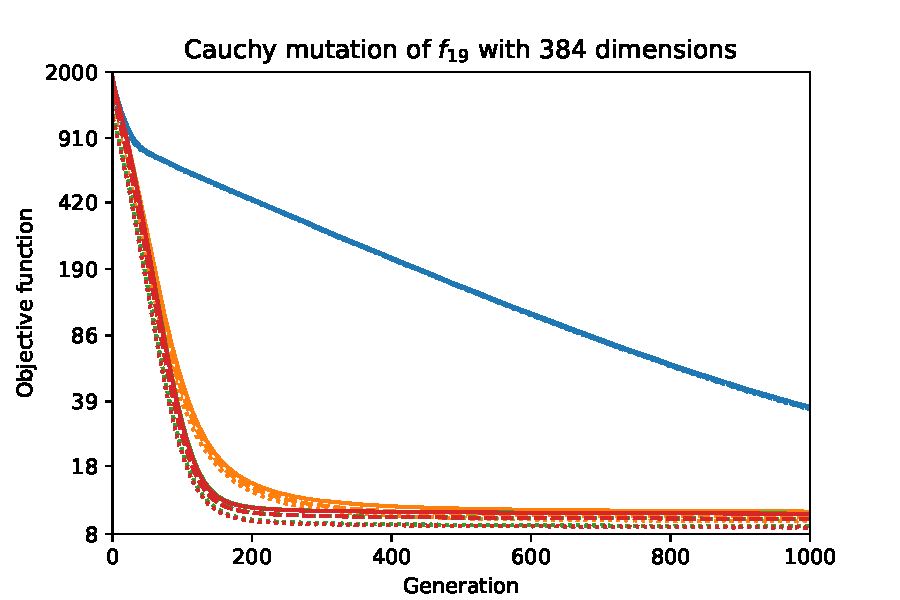
\includegraphics[width=\textwidth]{img/runs/fitness_es_mutation_f19_dim384_AddFromCauchy.pdf}
    \end{minipage}

    \begin{minipage}[t]{0.32\textwidth}
        \centering
        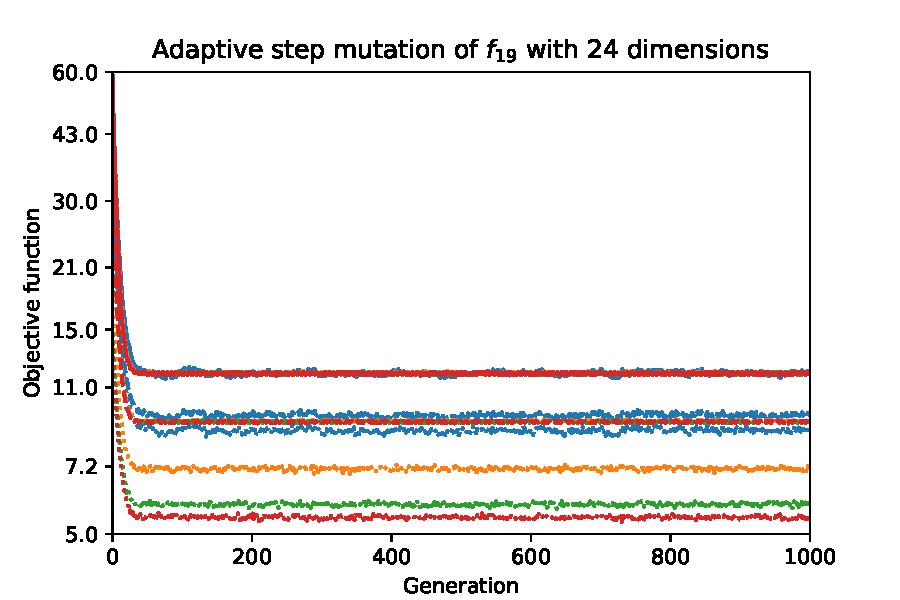
\includegraphics[width=\textwidth]{img/runs/fitness_es_mutation_f19_dim24_AdaptiveStep.pdf}
    \end{minipage}
    \hfill
    \begin{minipage}[t]{0.32\textwidth}
        \centering
        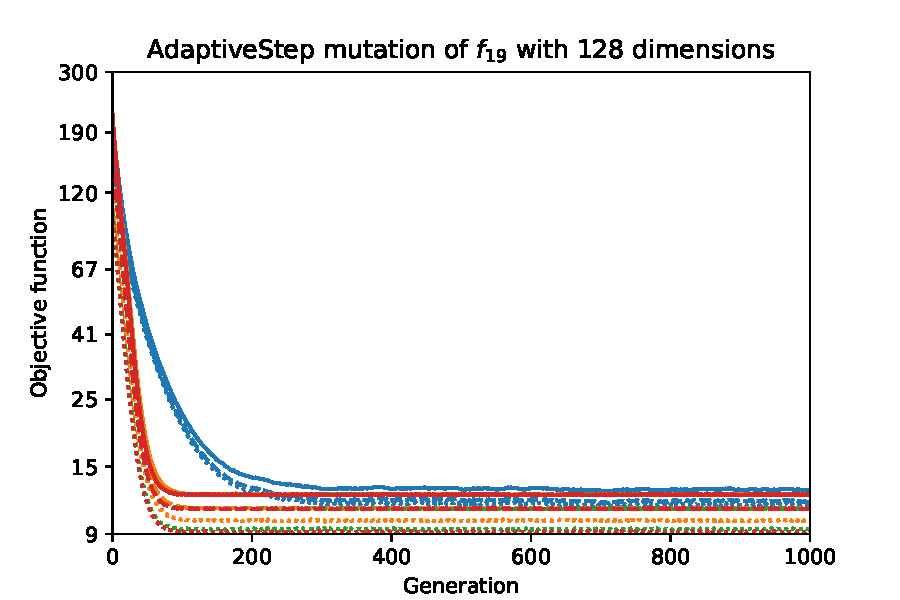
\includegraphics[width=\textwidth]{img/runs/fitness_es_mutation_f19_dim128_AdaptiveStep.pdf}
    \end{minipage}
    \hfill
    \begin{minipage}[t]{0.32\textwidth}
        \centering
        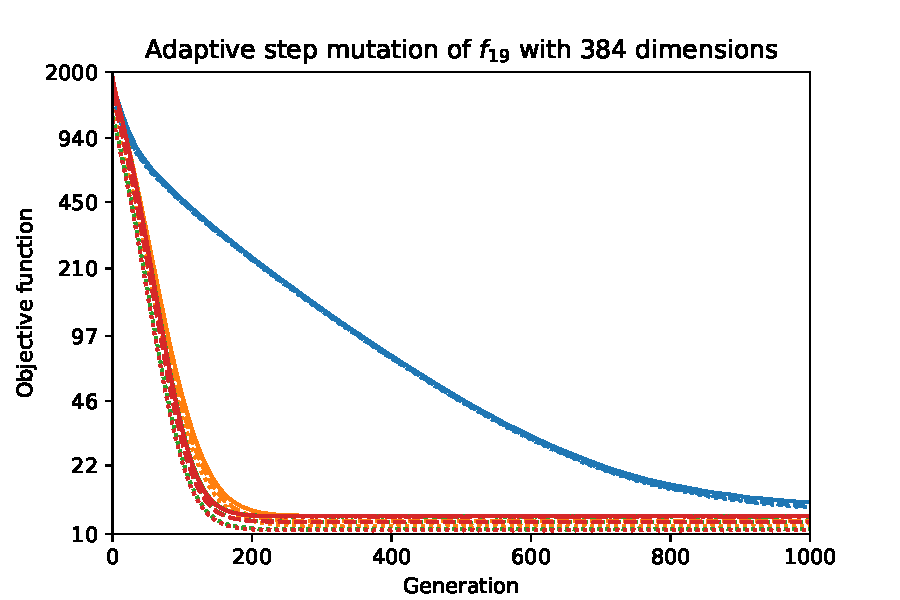
\includegraphics[width=\textwidth]{img/runs/fitness_es_mutation_f19_dim384_AdaptiveStep.pdf}
    \end{minipage}

    \begin{minipage}{\textwidth}
        \centering
        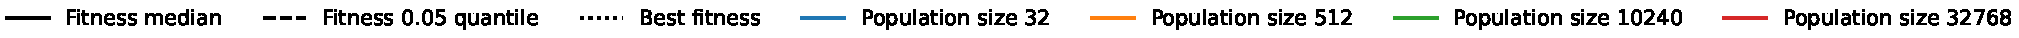
\includegraphics[width=\textwidth]{img/runs/fitness_es_mutation_legend.pdf}
    \end{minipage}

    \caption[Fitness of various mutation operators in real--coded evolutionary algorithms]{Fitness of real--coded evolutionary algorithm with various mutation operators. Measured on \acrshort{acc:bbob} functions $f_{19}$ and $f_{24}$ (available in attachments). Algorithm used hyperparameters specified in table \ref{tab:esmutationhyperparmarameters}.}
    \label{meas:mutfitness}
\end{figure}



%%%%%%%%%%%%%%%%%%%%%%%
%%                   %%
%%   ES CROSSOVERS   %%
%%                   %%
%5%%%%%%%%%%%%%%%%%%%%%
\begin{figure}[ht!]
    \begin{minipage}[t]{0.32\textwidth}
        \centering
        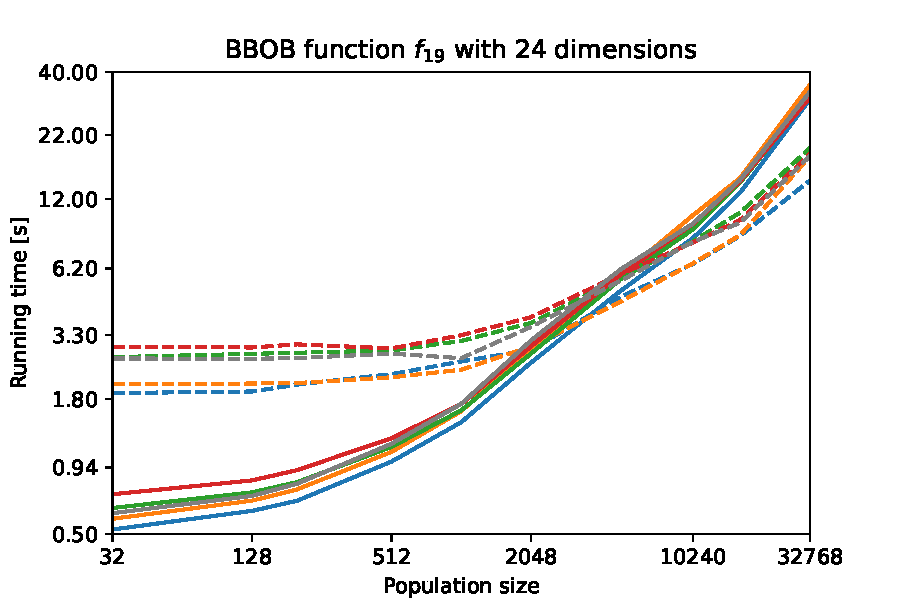
\includegraphics[width=\textwidth]{img/runs/time_es_crossover_fn19_24d.pdf}
    \end{minipage}
    \hfill
    \begin{minipage}[t]{0.32\textwidth}
        \centering
        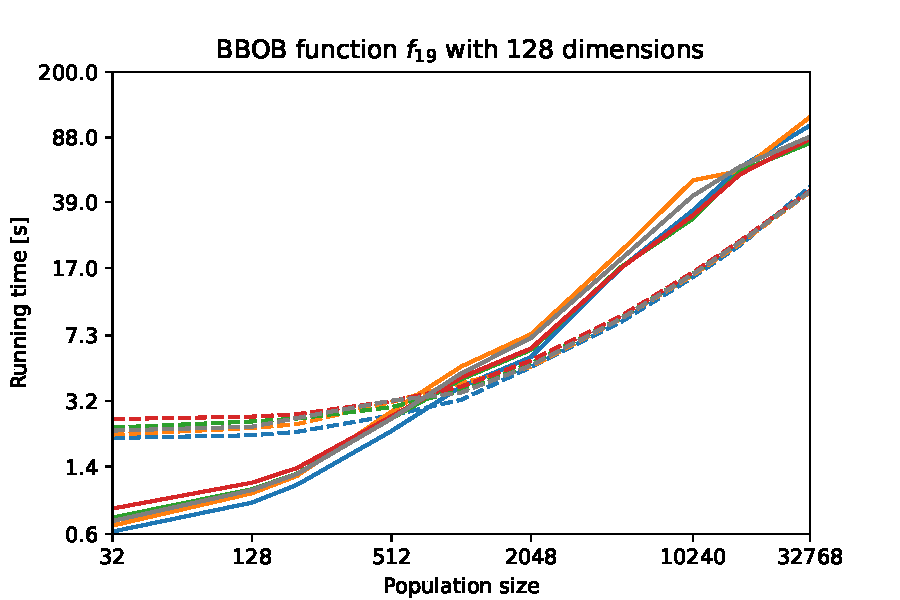
\includegraphics[width=\textwidth]{img/runs/time_es_crossover_fn19_128d.pdf}
    \end{minipage}
    \hfill
    \begin{minipage}[t]{0.32\textwidth}
        \centering
        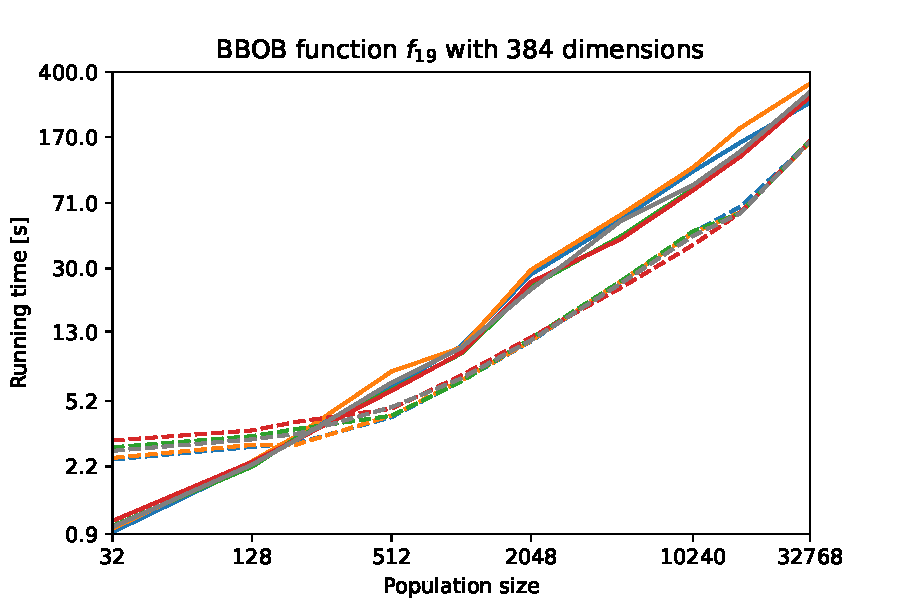
\includegraphics[width=\textwidth]{img/runs/time_es_crossover_fn19_384d.pdf}
    \end{minipage}

    \begin{minipage}[t]{0.32\textwidth}
        \centering
        \includegraphics[width=\textwidth]{img/runs/time_es_crossover_fn24_24d.pdf}
    \end{minipage}
    \hfill
    \begin{minipage}[t]{0.32\textwidth}
        \centering
        \includegraphics[width=\textwidth]{img/runs/time_es_crossover_fn24_128d.pdf}
    \end{minipage}
    \hfill
    \begin{minipage}[t]{0.32\textwidth}
        \centering
        \includegraphics[width=\textwidth]{img/runs/time_es_crossover_fn24_384d.pdf}
    \end{minipage}

    \begin{minipage}{\textwidth}
        \centering
        \includegraphics[width=\textwidth]{img/runs/time_es_crossover_legend.pdf}
    \end{minipage}

    \caption[Running time of crossover operators]{Running time of real--coded evolutionary algorithm with various crossover operators. I chose to measure only \acrshort{acc:bbob} functions $f_{19}$ and $f_{24}$. Algorithm used hyperparameters specified in table \ref{tab:escrossoverhyperparmarameters} and run for $1000$ generations.}
    \label{meas:crosstime}
\end{figure}


\begin{figure}[ht!]
    \begin{minipage}[t]{0.32\textwidth}
        \centering
        \includegraphics[width=\textwidth]{img/runs/fitness_es_crossover_f19_dim24_Arithmetic.pdf}
    \end{minipage}
    \hfill
    \begin{minipage}[t]{0.32\textwidth}
        \centering
        \includegraphics[width=\textwidth]{img/runs/fitness_es_crossover_f19_dim24_Blend.pdf}
    \end{minipage}
    \hfill
    \begin{minipage}[t]{0.32\textwidth}
        \centering
        \includegraphics[width=\textwidth]{img/runs/fitness_es_crossover_f19_dim24_Uniform.pdf}
    \end{minipage}
    \\
    \centering
    \begin{minipage}[t]{0.32\textwidth}
        \includegraphics[width=\textwidth]{img/runs/fitness_es_crossover_f19_dim24_OnePoint1D.pdf}
    \end{minipage}
    \begin{minipage}[t]{0.32\textwidth}
        \centering
        \includegraphics[width=\textwidth]{img/runs/fitness_es_crossover_f19_dim24_TwoPoint1D.pdf}
    \end{minipage}

        \begin{minipage}[t]{0.32\textwidth}
        \centering
        \includegraphics[width=\textwidth]{img/runs/fitness_es_crossover_f24_dim384_Arithmetic.pdf}
    \end{minipage}
    \hfill
    \begin{minipage}[t]{0.32\textwidth}
        \centering
        \includegraphics[width=\textwidth]{img/runs/fitness_es_crossover_f24_dim384_Blend.pdf}
    \end{minipage}
    \hfill
    \begin{minipage}[t]{0.32\textwidth}
        \centering
        \includegraphics[width=\textwidth]{img/runs/fitness_es_crossover_f24_dim384_Uniform.pdf}
    \end{minipage}
    \\
    \centering
    \begin{minipage}[t]{0.32\textwidth}
        \includegraphics[width=\textwidth]{img/runs/fitness_es_crossover_f24_dim384_OnePoint1D.pdf}
    \end{minipage}
    \begin{minipage}[t]{0.32\textwidth}
        \centering
        \includegraphics[width=\textwidth]{img/runs/fitness_es_crossover_f24_dim384_TwoPoint1D.pdf}
    \end{minipage}

    \begin{minipage}{\textwidth}
        \centering
        \includegraphics[width=\textwidth]{img/runs/fitness_es_crossovers_legend.pdf}
    \end{minipage}

    \caption[Fitness of various crossover operators in real--coded evolutionary algorithms]{Fitness of real--coded evolutionary algorithm with various crossover operators. Measured only on \acrshort{acc:bbob} functions $f_{19}$ and $f_{24}$ with dimensions $24$, $128$, and $384$. Algorithm used hyperparameters specified in table \ref{tab:escrossoverhyperparmarameters}. I present only function $f_{19}$ with $24$ dimensions and function $f_{24}$ with $384$ dimensions, rest of the measurements are in the attachments.}
    \label{meas:crossfitness}
\end{figure}




%%%%%%%%%%%%%%%%%%%
%%               %%
%%   ES SCHEMA   %%
%%               %%
%5%%%%%%%%%%%%%%%%%
\begin{figure}[ht!]
    \begin{minipage}[t]{0.32\textwidth}
        \centering
        \includegraphics[width=\textwidth]{img/runs/time_es_schema_fn19_24d.pdf}
    \end{minipage}
    \hfill
    \begin{minipage}[t]{0.32\textwidth}
        \centering
        \includegraphics[width=\textwidth]{img/runs/time_es_schema_fn19_128d.pdf}
    \end{minipage}
    \hfill
    \begin{minipage}[t]{0.32\textwidth}
        \centering
        \includegraphics[width=\textwidth]{img/runs/time_es_schema_fn19_384d.pdf}
    \end{minipage}

    \begin{minipage}[t]{0.32\textwidth}
        \centering
        \includegraphics[width=\textwidth]{img/runs/time_es_schema_fn22_24d.pdf}
    \end{minipage}
    \hfill
    \begin{minipage}[t]{0.32\textwidth}
        \centering
        \includegraphics[width=\textwidth]{img/runs/time_es_schema_fn22_128d.pdf}
    \end{minipage}
    \hfill
    \begin{minipage}[t]{0.32\textwidth}
        \centering
        \includegraphics[width=\textwidth]{img/runs/time_es_schema_fn22_384d.pdf}
    \end{minipage}

    \begin{minipage}{\textwidth}
        \centering
        \includegraphics[width=0.6\textwidth]{img/runs/time_es_schema_legend.pdf}
    \end{minipage}

    \caption[Running time of crossover schemas]{Running time of real--coded evolutionary algorithm with various crossover schemas. I measure the algorithm on \acrshort{acc:bbob} functions $f_{19}$ and $f_{22}$ with $24$, $128$, and $384$ dimensions. Algorithm used hyperparameters specified in table \ref{tab:esschemehyperparmarameters} and run for $1000$ generations.}
    \label{meas:schema}
\end{figure}




%%%%%%%%%%%%%%%%%
%%             %%
%%   PSO2006   %%
%%             %%
%%%%%%%%%%%%%%%%%
\begin{figure}[ht!]
    \begin{minipage}[t]{0.32\textwidth}
        \centering
        \includegraphics[width=\textwidth]{img/runs/time_pso2006_fn1_alldim.pdf}
    \end{minipage}
    \hfill
    \begin{minipage}[t]{0.32\textwidth}
        \centering
        \includegraphics[width=\textwidth]{img/runs/time_pso2006_fn7_alldim.pdf}
    \end{minipage}
    \hfill
    \begin{minipage}[t]{0.32\textwidth}
        \centering
        \includegraphics[width=\textwidth]{img/runs/time_pso2006_fn15_alldim.pdf}
    \end{minipage}

    \begin{minipage}[t]{0.32\textwidth}
        \centering
        \includegraphics[width=\textwidth]{img/runs/time_pso2006_fn19_alldim.pdf}
    \end{minipage}
    \hfill
    \begin{minipage}[t]{0.32\textwidth}
        \centering
        \includegraphics[width=\textwidth]{img/runs/time_pso2006_fn22_alldim.pdf}
    \end{minipage}
    \hfill
    \begin{minipage}[t]{0.32\textwidth}
        \centering
        \includegraphics[width=\textwidth]{img/runs/time_pso2006_fn24_alldim.pdf}
    \end{minipage}

    \begin{minipage}{\textwidth}
        \centering
        \includegraphics[width=\textwidth]{img/runs/time_pso2006_alldim_legend.pdf}
    \end{minipage}

    \caption[Running time of PSO2006]{Running time of \acrlong{acc:spso2006} algorithm using problems of dimension $6$, $32$, $128$, and $384$. The algorithm run for $1000$ generations. Populations with over $1000$ particles takes advantage of \gpu and are clearly faster to evaluate.}
    \label{meas:spso2006time}
\end{figure}

\begin{figure}[ht!]
    \begin{minipage}[t]{0.32\textwidth}
        \centering
        \includegraphics[width=\textwidth]{img/runs/fitness_pso2006_f1.pdf}
    \end{minipage}
    \hfill
    \begin{minipage}[t]{0.32\textwidth}
        \centering
        \includegraphics[width=\textwidth]{img/runs/fitness_pso2006_f7.pdf}
    \end{minipage}
    \hfill
    \begin{minipage}[t]{0.32\textwidth}
        \centering
        \includegraphics[width=\textwidth]{img/runs/fitness_pso2006_f15.pdf}
    \end{minipage}

    \begin{minipage}[t]{0.32\textwidth}
        \centering
        \includegraphics[width=\textwidth]{img/runs/fitness_pso2006_f19.pdf}
    \end{minipage}
    \hfill
    \begin{minipage}[t]{0.32\textwidth}
        \centering
        \includegraphics[width=\textwidth]{img/runs/fitness_pso2006_f22.pdf}
    \end{minipage}
    \hfill
    \begin{minipage}[t]{0.32\textwidth}
        \centering
        \includegraphics[width=\textwidth]{img/runs/fitness_pso2006_f24.pdf}
    \end{minipage}

    \begin{minipage}{\textwidth}
        \centering
        \includegraphics[width=\textwidth]{img/runs/fitness_pso2006_legend.pdf}
    \end{minipage}

    \caption[Fitness of PSO2006 algorithm]{Median, $0.05$ quantile, and best fitness of \acrlong{acc:spso2006} algorithm using random neighborhood on problem with $128$ dimensions. I measured populations consisting of $32$, $512$, $10240$, and $32768$ particles. All the problem functions take advantage of more particles, except of function $f_7$. Given hyperparameters in table \ref{tab:psohyperparameters}, \acrshort{acc:spso2006} seems to have better convergence properties in comparison to \acrshort{acc:spso2011}.}
    \label{meas:spso2006fitness}
\end{figure}




%%%%%%%%%%%%%%%%%%%%%%%%%%
%%                      %%
%%   PSO NEIGHBORHOOD   %%
%%                      %%
%%%%%%%%%%%%%%%%%%%%%%%%%%
\begin{figure}[ht!]
    \begin{minipage}[t]{0.32\textwidth}
        \centering
        \includegraphics[width=\textwidth]{img/runs/time_pso2006_fn1_neigh.pdf}
    \end{minipage}
    \hfill
    \begin{minipage}[t]{0.32\textwidth}
        \centering
        \includegraphics[width=\textwidth]{img/runs/time_pso2006_fn7_neigh.pdf}
    \end{minipage}
    \hfill
    \begin{minipage}[t]{0.32\textwidth}
        \centering
        \includegraphics[width=\textwidth]{img/runs/time_pso2006_fn15_neigh.pdf}
    \end{minipage}

    \begin{minipage}[t]{0.32\textwidth}
        \centering
        \includegraphics[width=\textwidth]{img/runs/time_pso2006_fn19_neigh.pdf}
    \end{minipage}
    \hfill
    \begin{minipage}[t]{0.32\textwidth}
        \centering
        \includegraphics[width=\textwidth]{img/runs/time_pso2006_fn22_neigh.pdf}
    \end{minipage}
    \hfill
    \begin{minipage}[t]{0.32\textwidth}
        \centering
        \includegraphics[width=\textwidth]{img/runs/time_pso2006_fn24_neigh.pdf}
    \end{minipage}

    \begin{minipage}{\textwidth}
        \centering
        \includegraphics[width=0.6\textwidth]{img/runs/time_pso_neigh_legend.pdf}
    \end{minipage}

    \caption[PSO2006 neighborhood running time]{Running time of \acrlong{acc:spso2006} algorithm with different neighborhood types. The algorithm run for 1000 generations on problem with 128 dimensions. Neighborhood sizes are at table \ref{tab:psohyperparameters}. The nearest neighborhood topology was run only to population of size 4900, as it compares all pairs of individuals and the device does not have enough memory. The minimum population size for grid topologies were 225, because topologies size were specified as a fraction of population size and for smaller populations neighborhood could not be constructed. The grid topologies were always assembled into square. Running times of circle, linear grid, compact grid, and diamond grid were almost identical (depending only on the size of neighborhood, see chapter \ref{chap:impl}), so I plot only measurements for circle and diamond grid.}
    \label{meas:psoneigtime}
\end{figure}



\begin{figure}[ht!]
    \begin{minipage}[t]{0.32\textwidth}
        \centering
        \includegraphics[width=\textwidth]{img/runs/fitness_pso_f24_neighRandom.pdf}
    \end{minipage}
    \hfill
    \begin{minipage}[t]{0.32\textwidth}
        \centering
        \includegraphics[width=\textwidth]{img/runs/fitness_pso_f24_neighNearest.pdf}
    \end{minipage}
    \hfill
    \begin{minipage}[t]{0.32\textwidth}
        \centering
        \includegraphics[width=\textwidth]{img/runs/fitness_pso_f24_neighCircle.pdf}
    \end{minipage}

    \begin{minipage}[t]{0.32\textwidth}
        \centering
        \includegraphics[width=\textwidth]{img/runs/fitness_pso_f24_neighLinearGrid.pdf}
    \end{minipage}
    \hfill
    \begin{minipage}[t]{0.32\textwidth}
        \centering
        \includegraphics[width=\textwidth]{img/runs/fitness_pso_f24_neighCompactGrid.pdf}
    \end{minipage}
    \hfill
    \begin{minipage}[t]{0.32\textwidth}
        \centering
        \includegraphics[width=\textwidth]{img/runs/fitness_pso_f24_neighDiamondGrid.pdf}
    \end{minipage}

    \begin{minipage}{\textwidth}
        \centering
        \includegraphics[width=0.8\textwidth]{img/runs/fitness_pso_neigh_legend.pdf}
    \end{minipage}

    \caption[Fitness of PSO neighborhoods]{Fitness of neighborhoods using $121$, $529$, $4900$, and $22500$ particles and \acrshort{acc:spso2006} update algorithm. Nearest neighborhood for $22500$ particles is not present, because of the memory demands. Grid neighborhoods for $121$ particles is not present, because there was not enough particles to build it. 
    All the neighborhoods clearly benefit from greater number of particles with the exception of compact grid and diamond grid. This is probably caused by premature convergence rather than degredation of the performance.
    Measurements for \acrshort{acc:bbob} functions $f_1$, $f_7$, $f_{15}$, and $f_{22}$ report similar properties.}
    \label{meas:psoneigfitness}
\end{figure}




%%%%%%%%%%%%%%%%%
%%             %%
%%   PSO2011   %%
%%             %%
%%%%%%%%%%%%%%%%%
\begin{figure}[ht!]
    \begin{minipage}[t]{0.32\textwidth}
        \centering
        \includegraphics[width=\textwidth]{img/runs/time_pso2011_fn1_alldim.pdf}
    \end{minipage}
    \hfill
    \begin{minipage}[t]{0.32\textwidth}
        \centering
        \includegraphics[width=\textwidth]{img/runs/time_pso2011_fn7_alldim.pdf}
    \end{minipage}
    \hfill
    \begin{minipage}[t]{0.32\textwidth}
        \centering
        \includegraphics[width=\textwidth]{img/runs/time_pso2011_fn15_alldim.pdf}
    \end{minipage}

    \begin{minipage}[t]{0.32\textwidth}
        \centering
        \includegraphics[width=\textwidth]{img/runs/time_pso2011_fn19_alldim.pdf}
    \end{minipage}
    \hfill
    \begin{minipage}[t]{0.32\textwidth}
        \centering
        \includegraphics[width=\textwidth]{img/runs/time_pso2011_fn22_alldim.pdf}
    \end{minipage}
    \hfill
    \begin{minipage}[t]{0.32\textwidth}
        \centering
        \includegraphics[width=\textwidth]{img/runs/time_pso2011_fn24_alldim.pdf}
    \end{minipage}

    \begin{minipage}{\textwidth}
        \centering
        \includegraphics[width=\textwidth]{img/runs/time_pso2011_alldim_legend.pdf}
    \end{minipage}

    \caption[Running time of PSO2011]{Running time of \acrlong{acc:spso2011} algorithm using problems of dimension $6$, $32$, $128$, and $384$. The algorithm run for $1000$ generations. Populations with over $1000$ particles takes clear advantage of \gpu.}
    \label{meas:spso2011time}
\end{figure}

\begin{figure}[ht!]
    \begin{minipage}[t]{0.32\textwidth}
        \centering
        \includegraphics[width=\textwidth]{img/runs/fitness_pso2011_f1.pdf}
    \end{minipage}
    \hfill
    \begin{minipage}[t]{0.32\textwidth}
        \centering
        \includegraphics[width=\textwidth]{img/runs/fitness_pso2011_f7.pdf}
    \end{minipage}
    \hfill
    \begin{minipage}[t]{0.32\textwidth}
        \centering
        \includegraphics[width=\textwidth]{img/runs/fitness_pso2011_f15.pdf}
    \end{minipage}

    \begin{minipage}[t]{0.32\textwidth}
        \centering
        \includegraphics[width=\textwidth]{img/runs/fitness_pso2011_f19.pdf}
    \end{minipage}
    \hfill
    \begin{minipage}[t]{0.32\textwidth}
        \centering
        \includegraphics[width=\textwidth]{img/runs/fitness_pso2011_f22.pdf}
    \end{minipage}
    \hfill
    \begin{minipage}[t]{0.32\textwidth}
        \centering
        \includegraphics[width=\textwidth]{img/runs/fitness_pso2011_f24.pdf}
    \end{minipage}

    \begin{minipage}{\textwidth}
        \centering
        \includegraphics[width=\textwidth]{img/runs/fitness_pso2011_legend.pdf}
    \end{minipage}

    \caption[Fitness of PSO2011 algorithm]{Median, $0.05$ quantile, and best fitness of \acrlong{acc:spso2011} algorithm using random neighborhood on problem with $128$ dimensions. I measured populations consisting of $32$, $512$, $10240$, and $32768$ particles. All the problem functions take advantage of more particles.}
    \label{meas:spso2011fitness}
\end{figure}